%%%%%%%% ICML 2022 EXAMPLE LATEX SUBMISSION FILE %%%%%%%%%%%%%%%%%

\documentclass[nohyperref]{article}

% Recommended, but optional, packages for figures and better typesetting:
\usepackage{xcolor}
\usepackage{microtype}
\usepackage{graphicx}
\usepackage{subfigure}
\usepackage{booktabs} % for professional tables
\usepackage{tcolorbox}
\usepackage{listings}
\usepackage{xspace}
\lstset{
basicstyle=\scriptsize\ttfamily,
frame=single,
backgroundcolor=\xcolor{light-gray}
}
% hyperref makes hyperlinks in the resulting PDF.
% If your build breaks (sometimes temporarily if a hyperlink spans a page)
% please comment out the following usepackage line and replace
% \usepackage{icml2022} with \usepackage[nohyperref]{icml2022} above.
\usepackage{hyperref}


% Attempt to make hyperref and algorithmic work together better:
\newcommand{\theHalgorithm}{\arabic{algorithm}}

% Use the following line for the initial blind version submitted for review:
%\usepackage{icml2022}

% If accepted, instead use the following line for the camera-ready submission:
\usepackage[accepted]{icml2022}

% For theorems and such
\usepackage{amsmath}
\usepackage{amssymb}
\usepackage{mathtools}
\usepackage{amsthm}
\usepackage{listings}
\usepackage{comment}

% if you use cleveref..
\usepackage[capitalize,noabbrev]{cleveref}

\usepackage{tikz}
\usetikzlibrary{bayesnet}

% \lstdefineformat{R}{~=\( \sim \)}

%%%%%%%%%%%%%%%%%%%%%%%%%%%%%%%%
% Technical terms
%%%%%%%%%%%%%%%%%%%%%%%%%%%%%%%%
\newcommand{\cascade}{cascade\xspace}
\newcommand{\cascades}{cascades\xspace}
\newcommand{\Cascades}{Cascades\xspace}

%%%%%%%%%%%%%%%%%%%%%%%%%%%%%%%%
% THEOREMS
%%%%%%%%%%%%%%%%%%%%%%%%%%%%%%%%
\theoremstyle{plain}
\newtheorem{theorem}{Theorem}[section]
\newtheorem{proposition}[theorem]{Proposition}
\newtheorem{lemma}[theorem]{Lemma}
\newtheorem{corollary}[theorem]{Corollary}
\theoremstyle{definition}
\newtheorem{definition}[theorem]{Definition}
\newtheorem{assumption}[theorem]{Assumption}
\theoremstyle{remark}
\newtheorem{remark}[theorem]{Remark}

% Todonotes is useful during development; simply uncomment the next line
%    and comment out the line below the next line to turn off comments
%\usepackage[disable,textsize=tiny]{todonotes}
\usepackage[textsize=tiny]{todonotes}

\DeclareMathOperator*{\argmax}{\arg\!\max}

% The \icmltitle you define below is probably too long as a header.
% Therefore, a short form for the running title is supplied here:
\icmltitlerunning{Language Model Cascades}

\begin{document}

\twocolumn[
% \icmltitle{Language Models are Probabilistic Inference Programs}
\icmltitle{Language Model Cascades}
% \icmltitle{Probabilistic Inference over Language Model Programs}

% It is OKAY to include author information, even for blind
% submissions: the style file will automatically remove it for you
% unless you've provided the [accepted] option to the icml2022
% package.

% List of affiliations: The first argument should be a (short)
% identifier you will use later to specify author affiliations
% Academic affiliations should list Department, University, City, Region, Country
% Industry affiliations should list Company, City, Region, Country

% You can specify symbols, otherwise they are numbered in order.
% Ideally, you should not use this facility. Affiliations will be numbered
% in order of appearance and this is the preferred way.
\icmlsetsymbol{equal}{*}

\begin{icmlauthorlist}
\icmlauthor{David Dohan}{comp}
\icmlauthor{Winnie Xu}{comp}
\icmlauthor{Aitor Lewkowycz}{x}
\icmlauthor{Jacob Austin}{comp}
\icmlauthor{David Bieber}{comp}
\icmlauthor{Raphael Gontijo Lopes}{comp}
\icmlauthor{Yuhuai Wu}{comp}
\icmlauthor{Henryk Michalewski}{comp}
\icmlauthor{Rif A. Saurous}{comp}
\icmlauthor{Jascha Sohl-dickstein}{comp}
\icmlauthor{Kevin Murphy}{comp}
\icmlauthor{Charles Sutton}{comp}
\end{icmlauthorlist}

\icmlaffiliation{comp}{Google Research, Mountain View, United States}
\icmlaffiliation{x}{Alphabet, X, the Moonshot Factory}
% \icmlaffiliation{research}{Google Research, Mountain View, United States}

\icmlcorrespondingauthor{David Dohan}{david@ddohan.com}
\icmlcorrespondingauthor{Winnie Xu}{winniexu@cs.toronto.edu}

% You may provide any keywords that you
% find helpful for describing your paper; these are used to populate
% the "keywords" metadata in the PDF but will not be shown in the document
\icmlkeywords{Machine Learning, ICML}

\vskip 0.3in
]

\newcommand{\ddohan}[1]{\textcolor{green}{{[david: #1]}}}
\newcommand{\xwinxu}[1]{\textcolor{purple}{{[winnie: #1]}}}
\newcommand{\kevin}[1]{\textcolor{red}{{[kevin: #1]}}}
\newcommand{\rif}[1]{\textcolor{brown}{{[rif: #1]}}}
\newcommand{\aitor}[1]{\textcolor{cyan}{[aitor: #1]}}
\newcommand{\henryk}[1]{\textcolor{orange}{[henryk: #1]}}
\newcommand{\charles}[1]{\textcolor{purple}{[charles: #1]}}

\urlstyle{same}

% this must go after the closing bracket ] following \twocolumn[ ...

% This command actually creates the footnote in the first column
% listing the affiliations and the copyright notice.
% The command takes one argument, which is text to display at the start of the footnote.
% The \icmlEqualContribution command is standard text for equal contribution.
% Remove it (just {}) if you do not need this facility.


\printAffiliationsAndNotice{}  % leave blank if no need to mention equal contribution
%\printAffiliationsAndNotice{\icmlEqualContribution} % otherwise use the standard text.

% TODOs:
% \begin{itemize}
% % \item Tikz imag of the QTA case, with plate notation to demonst
% % \item Verifiers illustration
% % \item Settle on graphical notation (ladder? compressed ladder?)
% %\item Tool use illustration
% %\item Discuss masked modeling
% %\item Expand appendix
% \end{itemize}

\begin{abstract}
Prompted models have demonstrated impressive few-shot learning abilities.
Repeated interactions at test-time with a single model, or the composition of multiple models together, further expands capabilities. These compositions are probabilistic models, and may be expressed in the language of graphical models with random variables whose values are complex data types such as strings. Cases with control flow and dynamic structure require techniques from probabilistic programming, 
which allow implementing disparate model structures and inference strategies in a unified language.
We formalize several existing techniques from this perspective, including scratchpads / chain of thought, verifiers, STaR, selection-inference, and tool use. We refer to the resulting programs as \emph{language model \cascades}.
%Furthermore, the few shot learning abilities of large language models may be used to amortize inference across tasks.
\end{abstract}

\documentclass[11pt]{report}
\usepackage[margin=2cm]{geometry}
\usepackage{graphicx}
\usepackage{float}
\usepackage{times}
\usepackage{url}
\usepackage[dvipsnames]{xcolor}
\usepackage{hyperref}

\newcommand{\specialcell}[2][c]{\begin{tabular}[#1]{@{}c@{}}#2\end{tabular}}

\newcommand{\Gap}{\texorpdfstring{\hfill}{}}
\newcommand{\Rec}{\texorpdfstring{{\small\emph{\color{ccai-blue}{\fbox{High Leverage}}}}}{}}
\newcommand{\HighRisk}{\texorpdfstring{{\small\emph{\color{ccai-yellow-darker}{\fbox{Uncertain Impact}}}}}{}}
\newcommand{\Longterm}{\texorpdfstring{{\small\emph{\color{ccai-green}{\fbox{Long-term}}}}}{}}

\begin{document}

\begin{abstract}
Climate change is one of the greatest challenges facing humanity, and we, as machine learning experts, may wonder how we can help. Here we describe how machine learning can be a powerful tool in reducing greenhouse gas emissions and helping society adapt to a changing climate. From smart grids to disaster management, we identify high impact problems where existing gaps can be filled by machine learning, in collaboration with other fields. Our recommendations encompass exciting research questions as well as promising business opportunities. We call on the machine learning community to join the global effort against climate change.
\vskip .5in
\end{abstract}

\part*{Introduction}
The effects of climate change are increasingly visible.\footnote{For a layman's introduction to the topic of climate change, see \cite{romm2018climate, archer2010climate}.} Storms, droughts, fires, and flooding have become stronger and more frequent \cite{field2012managing}. Global ecosystems are changing, including the natural resources and agriculture on which humanity depends. The 2018 intergovernmental report on climate change estimated that the world will face catastrophic consequences unless global greenhouse gas emissions are eliminated within thirty years \cite{ipcc_global_2018}. Yet year after year, these emissions rise.

Addressing climate change involves mitigation (reducing emissions) and adaptation (preparing for unavoidable consequences). Both are multifaceted issues. Mitigation of greenhouse gas (GHG) emissions requires changes to electricity systems, transportation, buildings, industry, and land use. Adaptation requires planning for resilience and disaster management, given an understanding of climate and extreme events. Such a diversity of problems can be seen as an opportunity: there are many ways to have an impact.

In recent years, machine learning (ML) has been recognized as a broadly powerful tool for technological progress. Despite the growth of movements applying ML and AI to problems of societal and global good,\footnote{See the AI for social good movement (e.g.~\cite{hager2019artificial, berendt2019ai}), ML for the developing world~\cite{de2018machine}, the computational sustainability movement (e.g.~\cite{kelling2018computational, joppa2017case, lassig2016computational, gomes2009computational, dietterich2009machine}, the American Meteorological Society's Committee on AI Applications to Environmental Science, and the field of Climate Informatics (\url{www.climateinformatics.org}) \cite{Monteleoni2013chapter}, as well as the relevant survey papers \cite{faghmous2014big, kaack2019challenges, ford2016opinion}.} there remains the need for a concerted effort to identify how these tools may best be applied to tackle climate change. Many ML practitioners wish to act, but are uncertain how. On the other side, many fields have begun actively seeking input from the ML community.

This paper aims to provide an overview of where machine learning can be applied with high impact in the fight against climate change, through either effective engineering or innovative research. The strategies we highlight include climate mitigation and adaptation, as well as meta-level tools that enable other strategies. In order to maximize the relevance of our recommendations, we have consulted experts across many fields (see \hyperref[sec:acknowledgments]{{\small{Acknowledgments}}}) in the preparation of this paper.


\begin{table}
\begin{small}
\begin{center}
\begin{tabular}{l l l l l l l l l l l l}  \toprule
     \multicolumn{2}{l}{ }
         & \small{\rotatebox{90}{\parbox{2.2cm}{Causal\\inference}}}
         & \small{\rotatebox{90}{\parbox{2.2cm}{Computer\\vision}}}
         & \small{\rotatebox{90}{\parbox{2.2cm}{Interpretable\\models}}}
         & \small{\rotatebox{90}{NLP}}
         & \small{\rotatebox{90}{\parbox{2.2cm}{RL \& Control}}}
        %  & \small{\rotatebox{90}{Robotics}}
         & \small{\rotatebox{90}{\parbox{2.2cm}{Time-series analysis}}}
         & \small{\rotatebox{90}{\parbox{2.2cm}{Transfer\\learning}}}
         & \small{\rotatebox{90}{\parbox{2.2cm}{Uncertainty\\quantification}}}
         & \small{\rotatebox{90}{\parbox{2.2cm}{Unsupervised\\learning}}}
    \\ \midrule
    \rowcolor{ccai-blue-lightest}
    \multicolumn{2}{l}{1 \hyperref[sec:electricity-systems]{Electricity systems}} 
        & % Causal inf
        &  % Comp vision
        & % Interpretable ml
        & % nlp
        & % rl + control
        & % time series
        & % transfer
        & % UQ
        & \\% unsupervised \ref{sub
    & \hyperref[sec:electricity-lowCarbon]{Enabling low-carbon electricity}
        & % Causal inf
        & $\bullet$% Comp vision
        & $\bullet$% % Interpretable ml
        & % % nlp
        & $\bullet$%% rl + control
        & $\bullet$% % time series
        & % transfer
        & $\bullet$% % UQ
        & $\bullet$\\% unsupervised 
    & \hyperref[sec:electricity-currentSystemImpact]{Reducing current-system impacts}
        & % Causal inf
        & $\bullet$% Comp vision
        & % Interpretable ml
        & % nlp
        & % rl + control
        & $\bullet$% % time series
        & % transfer
        & $\bullet$% % UQ
        & $\bullet$\\% unsupervised 
    & \hyperref[sec:electricity-developing]{Ensuring global impact}
        & % Causal inf
        & $\bullet$% Comp vision
        & % Interpretable ml
        & % nlp
        & % rl + control
        & % time series
        & $\bullet$ % transfer
        & % UQ
        & $\bullet$\\% unsupervised 
    \rowcolor{ccai-blue-lightest}
    \multicolumn{2}{l}{2 \hyperref[sec:transportation]{Transportation}} 
        & % Causal inf
        & % Comp vision
        &% Interpretable ml
        & % nlp
        & % rl + control
        & % time series
        & % transfer
        & % UQ
        & \\% unsupervised 
    & \hyperref[sec:TReducing]{Reducing transport activity}
        & % Causal inf
        & $\bullet$% Comp vision
        & % Interpretable ml
        & % nlp
        & % rl + control
        & $\bullet$% time series
        & % transfer
        & $\bullet$% UQ
        & $\bullet$\\% unsupervised     
   & \hyperref[sec:TEfficient]{Improving vehicle efficiency}
        & % Causal inf
        & $\bullet$% Comp vision
        & % Interpretable ml
        & % nlp
        & $\bullet$% rl + control
        & % time series
        & % transfer
        & % UQ
        & \\% unsupervised    
   & \hyperref[sec:TFuels]{Alternative fuels \& electrification}
        & % Causal inf
        & % Comp vision
        & % Interpretable ml
        & % nlp
        & $\bullet$% rl + control
        & % time series
        & % transfer
        & % UQ
        & $\bullet$ \\% unsupervised    
   & \hyperref[sec:modalshift]{Modal shift}
        & $\bullet$% Causal inf
        & $\bullet$% Comp vision
        & % Interpretable ml
        & % nlp
        & % rl + control
        & $\bullet$% time series
        & % transfer
        & $\bullet$% UQ
        & \\% unsupervised    
    \rowcolor{ccai-blue-lightest}
    \multicolumn{2}{l}{3 \hyperref[sec:buildings-cities]{Buildings and cities}} 
        & % Causal inf
        & % Comp vision
        & % Interpretable ml
        & % nlp
        & % rl + control
        & % time series
        & % transfer
        & % UQ
        & \\% unsupervised 
    & \hyperref[sec:indv]{Optimizing buildings}
        & $\bullet$% Causal inf
        & % Comp vision
        & % Interpretable ml
        & % nlp
        & $\bullet$% rl + control
        & $\bullet$% time series
        & $\bullet$% transfer
        & % UQ
        & \\% unsupervised 
    & \hyperref[sec:distr]{Urban planning}
        & % Causal inf
        & $\bullet$% Comp vision
        & % Interpretable ml
        & % nlp
        & % rl + control
        & $\bullet$% time series
        & $\bullet$% transfer
        & % UQ
        & $\bullet$\\% unsupervised 
    & \hyperref[sec:cities]{The future of cities}
        & % Causal inf
        & % Comp vision
        & % Interpretable ml
        & $\bullet$%% nlp
        & % rl + control
        & %% time series
        & $\bullet$%% transfer
        & $\bullet$% UQ
        & $\bullet$\\% unsupervised 
    \rowcolor{ccai-blue-lightest}
    \multicolumn{2}{l}{4 \hyperref[sec:industry]{Industry}} 
        & % Causal inf
        & % Comp vision
        & % Interpretable ml
        & % nlp
        & % rl + control
        & % time series
        & % transfer
        & % UQ
        & \\% unsupervised 
    & \hyperref[sec:supplychains]{Optimizing supply chains}
        & % Causal inf
        & $\bullet$ %% Comp vision
        & % Interpretable ml
        & % nlp
        & $\bullet$ % rl + control
        & $\bullet$ % time series
        & % transfer
        & % UQ
        & \\% unsupervised 
    & \hyperref[sec:materialsandconstruction]{Improving materials}
        & %% Causal inf
        & % Comp vision
        & % Interpretable ml
        & % nlp
        & % rl + control
        & % time series
        & %% transfer
        & % UQ
        & $\bullet$ \\% unsupervised 
    & \hyperref[sec:demandresponse]{Production \& energy}
        & %% Causal inf
        & $\bullet$%% Comp vision
        & $\bullet$ %% Interpretable ml
        & % nlp
        & $\bullet$% rl + control
        & %% time series
        & %% transfer
        & % UQ
        & \\% unsupervised 
    \rowcolor{ccai-blue-lightest}
    \multicolumn{2}{l}{5 \hyperref[sec:afolu]{Farms \& forests}} 
        & % Causal inf
        & % Comp vision
        & % Interpretable ml
        & % nlp
        & % rl + control
        & % time series
        & % transfer
        & % UQ
        & \\% unsupervised 
    & \hyperref[sec:emissions-detection]{Remote sensing of emissions}
        & % Causal inf
        & $\bullet$% Comp vision
        & % Interpretable ml
        & % nlp
        & % rl + control
        & % time series
        & % transfer
        & % UQ
        & \\% unsupervised 
    & \hyperref[sec:agriculture]{Precision agriculture}
        & % Causal inf
        & $\bullet$% Comp vision
        & % Interpretable ml
        & % nlp
        & $\bullet$% rl + control
        & $\bullet$% time series
        & % transfer
        & % UQ
        & \\% unsupervised 
    & \hyperref[sec:peatlands]{Monitoring peatlands}
        & % Causal inf
        & $\bullet$% Comp vision
        & % Interpretable ml
        & % nlp
        & % rl + control
        & % time series
        & % transfer
        & % UQ
        & \\% unsupervised 
    & \hyperref[sec:forests]{Managing forests}
        & % Causal inf
        & $\bullet$% Comp vision
        & % Interpretable ml
        & % nlp
        & $\bullet$ % rl + control
        & $\bullet$ % time series
        & % transfer
        & % UQ
        & \\% unsupervised 
    \rowcolor{ccai-blue-lightest}
    \multicolumn{2}{l}{6 \hyperref[sec:ccs]{Carbon dioxide removal}}
        & % Causal inf
        & % Comp vision
        & % Interpretable ml
        & % nlp
        & % rl + control
        & % time series
        & % transfer
        & % UQ
        & \\
    & \hyperref[sec:ccs]{Direct air capture}
        & % Causal inf
        & % Comp vision
        & % Interpretable ml
        & % nlp
        & % rl + control
        & % time series
        & % transfer
        & % UQ
        & $\bullet$\\% unsupervised 
    & \hyperref[subsubsec: sequestrativervin]{Sequestering~\cd}
        & % Causal inf
        & $\bullet$% Comp vision
        & % Interpretable ml
        & % nlp
        & % rl + control
        & % time series
        & % transfer
        & $\bullet$% UQ
        & $\bullet$\\% unsupervised 
    \rowcolor{ccai-blue-lightest}
    \multicolumn{2}{l}{7 \hyperref[sec: climate prediction]{Climate prediction}} 
        & % Causal inf
        & % Comp vision
        & % Interpretable ml
        & % nlp
        & % rl + control
        & % time series
        & % transfer
        & % UQ
        & \\% unsupervised 
    & \hyperref[sec:climate-models-params]{Uniting data, ML \& climate science}
        & % Causal inf
        & $\bullet$% Comp vision
        & $\bullet$% Interpretable ml
        & % nlp
        & % rl + control
        & $\bullet$% time series
        & % transfer
        & $\bullet$% UQ
        & \\% unsupervised 
    & \hyperref[sec:models-extreme-events]{Forecasting extreme events}
        & % Causal inf
        & $\bullet$% Comp vision
        & $\bullet$% Interpretable ml
        & % nlp
        & % rl + control
        & $\bullet$% time series
        & % transfer
        & $\bullet$% UQ
        & \\% unsupervised 
    \rowcolor{ccai-blue-lightest}
    \multicolumn{2}{l}{8 \hyperref[sec:societal-impacts]{Societal impacts}} 
        & % Causal inf
        & % Comp vision
        & % Interpretable ml
        & % nlp
        & % rl + control
        & % time series
        & % transfer
        & % UQ
        & \\% unsupervised 
    & \hyperref[subsub:ecology]{Ecology}
        & % Causal inf
        & $\bullet$% Comp vision
        & % Interpretable ml
        & % nlp
        & % rl + control
        & % time series
        & $\bullet$% transfer
        & % UQ
        & \\% unsupervised 
    & \hyperref[subsub:infrastructure]{Infrastructure}
        & % Causal inf
        & % Comp vision
        & % Interpretable ml
        & % nlp
        & $\bullet$% rl + control
        & $\bullet$% time series
        & % transfer
        & $\bullet$% UQ
        & \\% unsupervised 
    & \hyperref[subsub:social_systems]{Social systems}
        & % Causal inf
        & $\bullet$% Comp vision
        & % Interpretable ml
        & % nlp
        & % rl + control
        & $\bullet$% time series
        & % transfer
        & % UQ
        & $\bullet$\\% unsupervised 
    & \hyperref[subsub:crisis]{Crisis}
        & % Causal inf
        & $\bullet$% Comp vision
        & % Interpretable ml
        & $\bullet$% nlp
        & % rl + control
        & % time series
        & % transfer
        & % UQ
        & \\% unsupervised 
    \rowcolor{ccai-blue-lightest}
    \multicolumn{2}{l}{9 \hyperref[sec:geoengineering]{Solar geoengineering}} 
        & % Causal inf
        & % Comp vision
        & % Interpretable ml
        & % nlp
        & % rl + control
        & % time series
        & % transfer
        & % UQ
        & \\% unsupervised 
    & \hyperref[subsub:better-aerosols]{Understanding \& improving aerosols}
        & % Causal inf
        & % Comp vision
        & % Interpretable ml
        & % nlp
        & % rl + control
        & $\bullet$% time series
        & % transfer
        & $\bullet$% UQ
        & \\% unsupervised 
    & \hyperref[subsub:planetary-control]{Engineering a planetary control system}
        & % Causal inf
        & % Comp vision
        & % Interpretable ml
        & % nlp
        & $\bullet$% rl + control
        & % time series
        & % transfer
        & $\bullet$% UQ
        & \\% unsupervised 
    & \hyperref[subsub:impact-models]{Modeling impacts}
        & % Causal inf
        & % Comp vision
        & % Interpretable ml
        & % nlp
        & % rl + control
        & $\bullet$% time series
        & % transfer
        & $\bullet$% UQ
        & \\% unsupervised 
    \rowcolor{ccai-blue-lightest}
    \multicolumn{2}{l}{10 \hyperref[sec:tools-individuals]{Individual action}} 
        & % Causal inf
        & % Comp vision
        & % Interpretable ml
        & % nlp
        & % rl + control
        & % time series
        & % transfer
        & % UQ
        & \\% unsupervised 
    & \hyperref[sec:personal_carbon_footprint]{Understanding personal footprint}
        & $\bullet$% Causal inf
        & % Comp vision
        & % Interpretable ml
        & $\bullet$% nlp
        & $\bullet$% rl + control
        & $\bullet$% time series
        & % transfer
        & % UQ
        & \\% unsupervised 
    & \hyperref[sec:behavior_change]{Facilitating behavior change}
        & % Causal inf
        & % Comp vision
        & % Interpretable ml
        & $\bullet$% nlp
        & % rl + control
        & % time series
        & % transfer
        & % UQ
        & $\bullet$\\% unsupervised 
    \rowcolor{ccai-blue-lightest}
    \multicolumn{2}{l}{11 \hyperref[sec:toolsforsociety]{Collective decisions}} 
        & % Causal inf
        & % Comp vision
        & % Interpretable ml
        & % nlp
        & % rl + control
        & % time series
        & % transfer
        & % UQ
        &  \\% unsupervised 
    & \hyperref[sec:coordination]{Modeling social interactions}
        & % Causal inf
        & % Comp vision
        & $\bullet$ % Interpretable ml
        & % nlp
        & $\bullet$ % rl + control
        & % time series
        & % transfer
        & % UQ
        & \\% unsupervised 
    & \hyperref[sec:decisionmaking]{Informing policy}
        & $\bullet$ % Causal inf
        & $\bullet$ % Comp vision
        & % Interpretable ml
        & $\bullet$% nlp
        & % rl + control
        & % time series
        & % transfer
        & $\bullet$% UQ
        & $\bullet$\\% unsupervised 
    & \hyperref[subsec:markets]{Designing markets}
        & % Causal inf
        & % Comp vision
        & % Interpretable ml
        & % nlp
        & $\bullet$% rl + control
        & $\bullet$% time series
        & % transfer
        & % UQ
        & $\bullet$\\% unsupervised 
    \rowcolor{ccai-blue-lightest}
    \multicolumn{2}{l}{12 \hyperref[sec:education]{Education}} 
        & % Causal inf
        & % Comp vision
        & % Interpretable ml
        & $\bullet$% nlp
        & $\bullet$% rl + control
        & % time series
        & % transfer
        & % UQ
        & \\% unsupervised 
    \rowcolor{ccai-blue-lightest}
    \multicolumn{2}{l}{13 \hyperref[sec:finance]{Finance}} 
        & % Causal inf
        & % Comp vision
        & % Interpretable ml
        & $\bullet$% nlp
        & % rl + control
        & $\bullet$% time series
        & % transfer
        & $\bullet$% UQ
        & \\% unsupervised 
    \bottomrule
\end{tabular}
\caption{Climate change solution domains, corresponding to sections of this paper, matched with selected areas of ML that are relevant to each. }
\label{tab:summary}
\end{center}
\end{small}
\end{table}


\subsection*{Who is this paper written for?}

We believe that our recommendations will prove valuable to several different audiences (detailed below). In our writing, we have assumed some familiarity with basic terminology in machine learning, but do not assume any prior familiarity with application domains (such as agriculture or electric grids).\\

\textbf{Researchers and engineers:}
We identify many problems that require conceptual innovation and can advance the field of ML, as well as being highly impactful. For example, we highlight how climate models afford an exciting domain for interpretable ML (see \S\ref{sec: climate prediction}).
We encourage researchers and engineers across fields to use their expertise in solving urgent problems relevant to society.\\

\textbf{Entrepreneurs and investors:} We identify many problems where existing ML techniques could have a major impact without further research, and where the missing piece is deployment. We realize that some of the recommendations we offer here will make valuable startups and nonprofits. For example, we highlight techniques for providing fine-grained solar forecasts for power companies (see \S\ref{sec:electricity-lowCarbon}), tools for helping reduce personal energy consumption (see \S\ref{sec:behavior_change}), and predictions for the financial impacts of climate change (see \S\ref{sec:finance}). We encourage entrepreneurs and investors to fill what is currently a wide-open space.\\

\textbf{Corporate leaders:} We identify problems where ML can lead to massive efficiency gains if adopted at scale by corporate players. For example, we highlight means of optimizing supply chains to reduce waste (see \S\ref{sec:supplychains}) and software/hardware tools for precision agriculture (see \S\ref{sec:agriculture}). We encourage corporate leaders to take advantage of opportunities offered by ML to benefit both the world and the bottom line.\\

\textbf{Local and national governments:} We identify problems where ML can improve public services, help gather data for decision-making, and guide plans for future development. For example, we highlight intelligent transportation systems (see \S\ref{sec:modalshift}), techniques for automatically assessing the energy consumption of buildings in cities (see \S\ref{sec:indv}),
and tools for improving disaster management (see \S\ref{subsub:crisis}). We encourage governments to consult ML experts while planning infrastructure and development, as this can lead to better, more cost-effective outcomes. We further encourage public entities to release data that may be relevant to climate change mitigation and adaptation goals.\\

\subsection*{How to read this paper} \label{sub:howtoread}
The paper is broken into sections according to application domain (see Table \ref{tab:summary}). To help the reader, we have also included the following flags at the level of individual strategies.
\begin{itemize}
\item \textbf{\Rec} $\,$ denotes bottlenecks that domain experts have identified in climate change mitigation or adaptation and that we believe to be particularly well-suited to tools from ML. These areas may be especially fruitful for ML practitioners wishing to have an outsized impact, though applications not marked with this flag are also valuable and should be pursued.
\item \textbf{\Longterm} $\,$ denotes applications that will have their primary impact after 2040. While extremely important, these may in some cases be less pressing than those which can help act on climate change in the near term.
\item \textbf{\HighRisk} $\,$ denotes applications where the impact on GHG emissions is uncertain (for example, the \emph{Jevons paradox} may apply\footnote{The Jevons paradox in economics refers to a situation where increased efficiency nonetheless results in higher overall demand. For example, autonomous vehicles could cause people to drive far more, so that overall GHG emissions could increase even if each ride is more efficient. In such cases, it becomes especially important to make use of specific policies, such as carbon pricing, to direct new technologies and the ML behind them. See also the literature on rebound effects and induced demand.}) or where there is  potential for undesirable side effects (\emph{negative externalities}).
\end{itemize}

These flags should not be taken as definitive; they represent our understanding of more rigorous analyses within the domains we consider, combined with our subjective evaluation of the potential role of ML in these various applications.

Despite the length of the paper, we cannot cover everything. There will certainly be many applications that we have not considered, or that we have erroneously dismissed. We look forward to seeing where future work leads.

\subsection*{A call for collaboration}

All of the problems we highlight in this paper require collaboration across fields. As the language used to refer to problems often varies between disciplines, we have provided keywords and background reading within each section of the paper. Finding collaborators and relevant data can sometimes be difficult; for additional resources, please visit the website that accompanies this paper: \url{https://www.climatechange.ai/}.

Collaboration makes it easier to develop effective strategies. Working with domain experts reduces the chance of using powerful tools when simple tools will do the job, of working on a problem that isn't actually relevant to practitioners, of overly simplifying a complex issue,
or of failing to anticipate risks.

Collaboration can also help ensure that new work reaches the audience that will use it. To be impactful, ML code should be accessible and published using a language and a platform that are already popular with the intended users. For maximal impact, new code can be integrated into an existing, widely used tool.

We emphasize that machine learning is not a silver bullet. The applications we highlight are impactful, but no one solution will ``fix'' climate change. There are also many areas of action where ML is inapplicable, and we omit these entirely. Furthermore, technology alone is not enough -- technologies that would address climate change have been available for years, but have largely not been adopted at scale by society. While we hope that ML will be useful in reducing the costs associated with climate action, humanity also must decide to act.

\end{document}

%!TEX root = ../main.tex

\section{Related Work}
\label{sec:related}

\textbf{State space models} have shown promise in modeling sequential data, including time series data~\citep{gu2022efficiently}, audio~\citep{goel2022s}, and visual data~\citep{nguyen2022s4nd}.
Our model builds off work on simplifying and parameterizing diagonal versions of S4~\citep{gu2022parameterization,gupta2022diagonal, gu2022train}.
Gated state spaces~\citep{mehta2022long} also aim to adapt SSMs to language modeling, but our results suggest that the GSS model does not perform as well as \hthree (or even as well as earlier SSMs like S4D).
The idea to combine SSMs with attention in hybrid models is not new; Mehta et al.~\citep{mehta2022long} also showed that interleaving attention with their GSS layer can improve performance, which we also validate on our OpenWebText experiments.
These positive results suggest that attention and SSMs are complementary, and that hybrid models may be a promising direction for future work.

\textbf{Large language foundation models}~\citep{bommasani2021opportunities} have demonstrated the power of scaling attention-based networks to billions of parameters and training them on trillions of tokens~\citep{hoffmann2022training}.
Understanding the mechanistic basis~\citep{elhage2021mathematical} behind these models may yield insights into better design choices for future models.
These and similar explorations have informed the design of \hthree and our selection of synthetic languages.
A number of recent works have also explored how to address the shortcomings of attention by approximating the attention computation~\citep{wang2020linformer,katharopoulos2020transformers, choromanski2020rethinking,tay2020long, kitaev2020reformer, daras2020smyrf}.
We believe these efforts are complementary to SSMs, and we are excited to see how they can be combined in future work.

\textbf{Linear attention}~\citep{katharopoulos2020transformers} and classical sequence models like RNNs serve as inspiration for \hthree.
Appendix~\ref{app:linear_attention} draws a direct connection between linear attention and LTI systems.
Luo et al.~\citep{luo2021stable} also propose a variant of linear attention that can achieve $O(n \log n)$ scaling in sequence length.
Appendix~\ref{sec:app_additional_experiments} evaluates linear attention on language modeling, and finds that it underperforms exact attention, whereas \hthree outperforms attention.
The multiplicative interactions in \hthree are reminiscent of gating mechanisms in LSTMs~\citep{hochreiter1996lstm} and GRUs~\citep{cho2014properties}, which suggests that architectural lessons from these sequence models may be useful for adapting SSMs to language modeling.
A number of algorithms for scaling attention to longer sequences have also been proposed, such as Transformer-XL~\citep{dai2019transformer}, Reformer~\citep{kitaev2020reformer}, Performer~\citep{choromanski2020rethinking}, and Perceiver AR~\citep{hawthorne2022general}.
Some of these approaches underperform exact attention on language modeling, and may be slower in wall-clock speed~\citep{dao2022flashattention}.
A thorough comparison of these alternatives to exact attention and how well they scale in model size and amount of training data is fruitful future work.

\textbf{FFT} algorithms are used in a wide variety of applications, including signal processing~\citep{oppenheim1978applications}, control theory~\citep{brogan1974modern}, and more.
Various algorithms for computing the FFT have existed for decades~\citep{oppenheim2001discrete}.
We hope our work on appealing to these classic algorithms to accelerate new applications such as learned SSMs will inspire future algorithmic exploration, even if hardware is not designed for them~\citep{hooker2021hardware}.

%%% Local Variables:
%%% mode: latex
%%% TeX-master: "../main"
%%% End:

\section{\Cascades}

In this section, we show how to create
\cascades\ of LMs to tackle various
language-based reasoning problems.
A \emph{\cascade} is a probabilistic program that includes
string-valued random variables, sampled from an LM.
For example, Figure~\ref{fig:cot_cascade} is a simple \cascade\ for question answering.
%For example, Figure~\ref{fig:si_cascade} is a simple \cascade\ for the selection-inference algorithm.
Each of the \texttt{yield} expressions return a string distributed according to the language model \texttt{S}.\footnote{The first argument
to \texttt{S} defines a unique name for the random variable,
and the remaining arguments conditions the LM on a string prefix. A variable may be marked as observed within the program, \texttt{S('varname', obs='observed value')}, or at inference time} This program defines a joint distribution over the variables \texttt{question, thought}, and \texttt{answer}.  Programs with complex control flow and observations are included in Appendix~\ref{app:implementation}.

We implement \cascades\ as a trace-based probabilistic programming language embedded in Python via effect handlers, inspired by \citet{pyro, numpyro}, and via coroutines, inspired by \citet{pymc4}. A pretrained LM is used to parameterize all conditional distributions. A \cascade supports arbitrary control flow and recursion. While the current presentation is in terms of few-shot prompting of causal language models, we emphasize that the ideas are immediately applicable to finetuned models, masked LM setting, and other complex data types including images.

\subsection{Scratchpads and Chain of thought}
\label{sec:QTA}

As our first example, we show how to 
 represent a chain of thought \citep{scratchpads, chainofthought} as shown in 
\cref{fig:QTA} and subsequent graphical model figures; refer to the corresponding probabilistic programs in \cref{app:implementation}.
We condition the $A$ node not just on the test question $Q$,
but also on previous $(Q^m,T^m,A^m)$ triples, which 
constitute the few-shot prompting part of the model.
This is denoted by the shaded nodes inside the plate.
Inference can be implemented by ancestral
sampling.

%
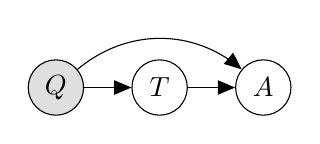
\begin{tikzpicture}
  % Define nodes
  \node[obs]           (Q) {$Q$};
  \node[latent, right=0.6cm of Q]         (T) {$T$};
  \node[latent, right=0.6cm of T]         (A) {$A$};

  % Connect the nodes
  \edge {Q} {T} ; %
  \edge {T} {A} ; %
  \draw [->] (Q) to [out=40,in=140] (A);
%   \path[every node/.style={font=\sffamily\small}]
%     (Q) edge[bend right] node [left] {} (A);
%   \edge[bend right=30] {Q} {A} ; %
\end{tikzpicture}
\begin{figure}[h!]
\centering
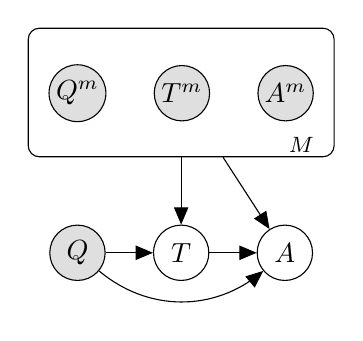
\begin{tikzpicture}
  % notation
  % [positioning] (name) {displayed name}
  

% Plate  
% Define nodes
\node[obs]           (Qf) {$Q^m$};
\node[obs, right=0.6cm of Qf]         (Tf) {$T^m$};
\node[obs, right=0.6cm of Tf]         (Af) {$A^m$};
%
%  % Connect the nodes
% \edge {Qf} {Tf} ; %
% \edge {Tf} {Af} ; %
% \draw [->] (Qf) to [out=40,in=140] (Af);
%  
\plate [inner sep=.25cm,yshift=.2cm] {fewshot} {(Qf)(Tf)(Af)} {$M$};

% Target task
%\node[obs]           (Q) {$Q$};
 \node[obs, below=1.3cm of Qf]           (Q) {$Q$};
\node[latent, right=0.6cm of Q]         (T) {$T$};
\node[latent, right=0.6cm of T]         (A) {$A$};
\edge {Q} {T} ; %
\edge {T} {A} ; %
\draw [->] (Q) to [out=-40,in=-140] (A);
  
  
% Connect plate to the 
\edge {fewshot} {T};
\edge {fewshot} {A};
\end{tikzpicture}
\caption{Question-Thought-Answer model.}
\label{fig:QTA}
\end{figure}



%In \cascades, we define the model in code in Figure~\ref{fig:cot_cascade}, where S is a (conditional) string distribution.
%The prompt for each variable is automatically constructed at inference time based on input variables and few shot examples.

% \charles{The program should not sample $q$, should it? Would it be more clear to leave off the 'question' etc arguments? Perhaps instead of question=q, we should use prefix=q, prefix=concat(q, t) to make it more generic? If we say this is a PPL, the reader is going to wonder whether we have observes. The program also does not explain how the prompt examples are used.}

% david: We can either say `S('question', obs='the question')`, or have the inference call inject the value (which is what I do in practice):
% `infer(program, observe(question='the question')`

% charles: Sure, the infer way is fine.  

% charles: I guess we can explain in the text that the first argument to S is a name for the r.v.

 % q = yield S('question')
  
\begin{figure}[h]
\begin{verbatim}
def qta():
  q = yield S('question')
  t = yield S('thought', question=q)
  a = yield S('answer', question=q, 
                        thought=t)
  return a
\end{verbatim}
\caption{Chain of thought \cascade\ in Python. Each \texttt{yield S(...)} statement samples a string from an LM. The name of the random variable is provided as the first argument to \texttt{S}.}
\label{fig:cot_cascade}
\end{figure}  

\subsection{Semi-supervised learning}
\label{sec:STAR}
In \cref{sec:QTA}, we provided a manually created set  $(Q^m,T^m,A^m)$ triples,
where the ``thoughts'' or ``rationalizations'' were provided.
A more scalable approach is to define a small set $D_S$
of such ``supervised'' triples,
but then to provide a larger set $D_L$ of $(Q^m,A^m)$ pairs,
which are easier to gather. % (e.g., by scraping question-answering web-sites).
We can augment the pairs in $D_L$ by adding 
the hidden $T^m$ variable to get a semi-supervised setup, shown in  
\cref{fig:QTAhidden}.

\begin{figure}[h!]
\centering
\begin{tikzpicture}
  % notation
  % [positioning] (name) {displayed name}
  
% Target task
\node[obs, below=0.8cm of fewshot]           (Q) {$Q$};
\node[latent, right=0.6cm of Q]         (T) {$T$};
\node[latent, right=0.6cm of T]         (A) {$A$};
\edge {Q} {T} ; %
\edge {T} {A} ; %
\draw [->] (Q) to [out=-40,in=-140] (A);
  
% Plate  
% Define nodes
\node[obs]           (Qf) {$Q^m$};
\node[latent, right=0.6cm of Qf]         (Tf) {$T^m$};
\node[obs, right=0.6cm of Tf]         (Af) {$A^m$};
%
%  % Connect the nodes
 \edge {Qf} {Tf} ; %
 \edge {Tf} {Af} ; %
% \draw [->] (Qf) to [out=40,in=140] (Af);
%  
\plate [inner sep=.25cm,yshift=.2cm] {fewshot} {(Qf)(Tf)(Af)} {$M$};

% Connect plate to the 
\edge {fewshot} {T};
\edge {fewshot} {A};
\end{tikzpicture}
\caption{QTA model with hidden thoughts.}
\label{fig:QTAhidden}
\end{figure}


The Self-Taught Reasoner (STaR) \citep{zelikman2022star} proposes a procedure for fine-tuning LMs in the chain-of-thought type setting.
We can interpret their method as a stochastic EM-like procedure in the cascade of \cref{fig:QTAhidden}.
In particular, they first fine-tune on the ``fully observed''
dataset $D_S = \{(Q^m,T^m,A^m)\}$.
Then they impute the unknown $T_i$ values in the 
``partially observed'' dataset  $D_L = \{(Q^m,T^m=?,A^m)\}$
during the ``E'' step by doing rejection sampling on $p(T, A | Q^m)$ until finding a thought which leads to the known correct answer. If sampling $(T,A)$ given the question fails to find the correct answer, they sample thoughts from $p(T | Q^m, A^m)$. This uses a recognition network to approximately sample from the posterior distribution over thoughts given the known correct answer.
%where the true answer is added to the prompt.
They call this approach  ``rationale generation with rationalization''. They then update the parameters in the ``M'' step based on these imputed thoughts.
By interpreting the rationale generation at this higher level of abstraction, we open up the possibility of applying this tuning method to other types of cascades.


%See \cref{sec:STAR} for details.

% We can fine-tune the model on this semi-supervised data
% using an EM-like procedure,
% as proposed for STaR (self-taught reasoner) \citep{zelikman2022star}.
% In the E step, they impute the unknown $T^m$ values in the $D_L$
% dataset, and in the M step, they update the LM parameters.
% 
% In the E step, thoughts are imputed by sampling from 
% $p(T | Q^m, A=A^m)$ using rejection sampling,
% where $p$ represents the language model,
% and they use $p(T,A|Q^m)$ as the proposal.
% If this fails to yield any correct answers,
% they use a more powerful proposal, 
%  $p(T,A|Q^m,A^m)$,
%  where the true answer is added to the prompt.
% They call this approach 
% ``rationale generation with rationalization''

%\input{star-old}

\subsection{Selection-Inference}
\label{sec:selection_inference}

Selection Inference \citep{selection_inference} is a recent example of multiple interacting LM modules. It proposes splitting reasoning into: the \textit{selection} module which selects a subset of facts given a question, and the \textit{inference} module which infers new facts given this subset.
%See \cref{sec:selection_inference} for details.

It may be represented by the model in \cref{fig:selective}. Here $S$ is the selection of a subset of ``facts''
from a pre-specified set of facts,
and $I$ is an inference driven by that fact.
The $S$ and $I$ nodes
can be iterated to do multistep reasoning.
The model is ``trained'' by giving it examples,
$D = \{ (Q^m, \{F^{mj}\}, S^m, I^m, A^m): m=1:M\}$,
as part of the prompt.
% It is then given a test question,
% and the answer is computed using
% $A \sim p(A|Q,D)$,
% ignoring (``marginalizing out'')\todo{ddohan: is this actually marginalizing out? It's just taking a single monte carlo sample by default. I would expect > 1 sample to marginalize}
% any intermediate $S$ or $I$ strings that
% might be generated by the model.

\begin{figure}[h!]
\centering
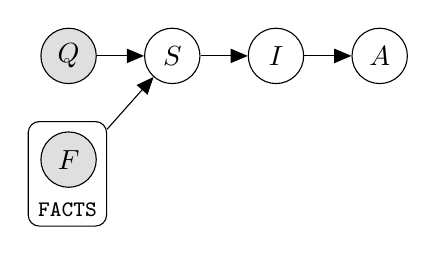
\begin{tikzpicture}
  % Define nodes
  \node[obs]           (Q) {$Q$};
  \node[obs, below=0.6cm of Q]           (F) {$F$};
  \plate{Fs} {
      (F)
  } {\texttt{FACTS}} %{$F \in \text{\texttt{FACTS}}$}
  \node[latent, right=0.6cm of Q]         (S) {$S$};
  \node[latent, right=0.6cm of S]         (I) {$I$};
  \node[latent, right=0.6cm of I]         (A) {$A$};

  % Connect the nodes
  \edge {Q,Fs} {S} ; %
  \edge {S} {I} ; %
  \edge {I} {A} ; %
  %\draw [->] (Q) to [out=40,in=140] (I);
  %\draw [->] (Q) to [out=40,in=140] (A);
%  \draw [->] (S) to [out=40,in=140] (A);
\end{tikzpicture}
\caption{Selection inference as a cascade. Here $S$ is the selected subset of facts and $I$ is an inference driven by this subset.}
\label{fig:selective}
\end{figure}

\subsection{Verifiers}
\label{sec:verifiers}

Although adding explicit ``thought'' variables to a model
has been found to improve performance, models still arrive at incorrect answers, or the correct answer for an erroneous reason.
An intuitive way to improve model performance is to train it to judge whether an answer and thought are likely to be ``valid''. \citet{verifiers} propose using a separate model as a verifier to filter solutions to reasoning tasks.
%sometimes
%these ``thoughts'' are erroneous,
%even though the answer may be correct.

We can create a ``labeled'' training
set of the form
$D = \{ (Q^m, T^m, A^m, V^m\}$,
where we add a ``verification'' label 
$V^m \in \{0, 1 \}$,
representing whether the thought $T^m$
is a valid form of reasoning for deriving
$A^m$ from $Q^m$, and $A^m$ is the correct answer.
This can be particularly helpful in settings
where there may be more than one way of deriving
the answer. The verifiers may be used to reject incorrect examples in ancestral sampling, and the thought generator may itself be conditioned on the verifiers being correct by finetuning or prompting, reminiscent of RL as inference \cite{rl_inference} and goal-conditioned policies such as decision-transformer \cite{decision_transformer}.

%\begin{figure}[h!]
\centering
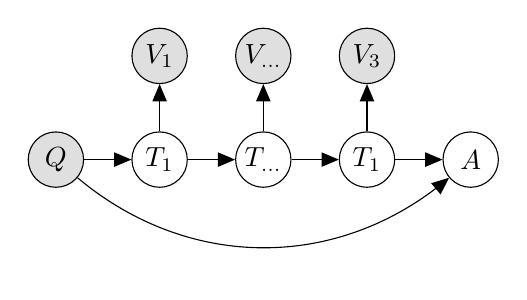
\begin{tikzpicture}
  % Define nodes
  \node[obs]           (Q) {$Q$};
  \node[latent, right=0.6cm of Q]         (T1) {$T_1$};
  \node[latent, right=0.6cm of T1]         (T2) {$T_{...}$};
  \node[latent, right=0.6cm of T2]         (T3) {$T_1$};
  \node[latent, right=0.6cm of T3]         (A) {$A$};
  
  \node[obs, above=0.6cm of T1]         (V1) {$V_1$};
  \node[obs, above=0.6cm of T2]         (V2) {$V_{...}$};
  \node[obs, above=0.6cm of T3]         (V3) {$V_3$};

  % Connect the nodes
  \edge {Q} {T1} ; %
  \edge {T1} {T2} ; %
  \edge {T2} {T3} ; %
  \edge {T3} {A} ; %
  \edge {T1} {V1} ; %
  \edge {T2} {V2} ; %
  \edge {T3} {V3} ; %
  \draw [->] (Q) to [out=-40,in=-140] (A);
%   \path[every node/.style={font=\sffamily\small}]
%     (Q) edge[bend right] node [left] {} (A);
%   \edge[bend right=30] {Q} {A} ; %
\end{tikzpicture}
\caption{The current way in which verifiers are diagrammed. Note that every node actually gets as input the concatenated strings of all of its parent nodes.}
\label{fig:verifier}
\end{figure}



%

\begin{figure}[h!]
\centering
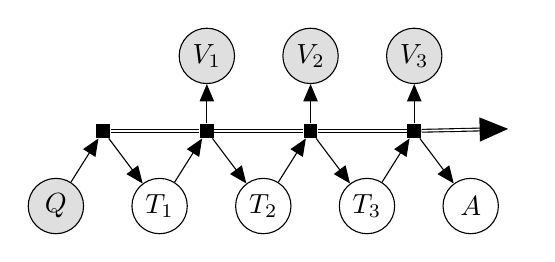
\begin{tikzpicture}
  % Define nodes
  \node[obs]    at (0,0)       (Q) {$Q$};

  \node[latent, right=0.6cm of Q]         (T1) {$T_1$};
  \node[latent, right=0.6cm of T1]         (T2) {$T_2$};
  \node[latent, right=0.6cm of T2]         (T3) {$T_3$};
  \node[latent, right=0.6cm of T3]         (A) {$A$};
  
  \node[factor, above=0.5cm of Q, xshift=0.6cm]       (stream1) {};
  \node[factor, above=0.5cm of T1, xshift=0.6cm]       (stream2) {};
  \node[factor, above=0.5cm of T2, xshift=0.6cm]       (stream3) {};
  \node[factor, above=0.5cm of T3, xshift=0.6cm]       (stream4) {};
  \node[above=0.5cm of A, xshift=0.6cm]       (stream5) {};
  
  \node[obs, above=0.5cm of stream2]         (V1) {$V_1$};
  \node[obs, above=0.5cm of stream3]         (V2) {$V_2$};
  \node[obs, above=0.5cm of stream4]         (V3) {$V_3$};


  % Connect the nodes
  \edge {Q} {stream1} ; %
  \edge {T1} {stream2} ; %
  \edge {T2} {stream3} ; %
  \edge {T3} {stream4} ; %
  \edge {stream1} {T1} ; %
  \edge {stream2} {T2} ; %
  \edge {stream3} {T3} ; %
  \edge {stream4} {A} ; %
  \draw [double] (stream1) to (stream2);
  \draw [double] (stream2) to (stream3);
  \draw [double] (stream3) to (stream4);
  \draw [double, ->] (stream4) to (stream5);

%   \edge {stream1} {stream2} ; %
%   \edge {stream2} {stream3} ; %
%   \edge {stream3} {stream4} ; %
%   \edge {stream4} {stream5} ; %
%   \edge {Q} {T1} ; %
%   \edge {T1} {T2} ; %
%   \edge {T2} {T3} ; %
%   \edge {T3} {A} ; %
  \edge {stream2} {V1} ; %
  \edge {stream3} {V2} ; %
  \edge {stream4} {V3} ; %
%   \draw [->] (Q) to [out=-40,in=-140] (A);
%   \path[every node/.style={font=\sffamily\small}]
%     (Q) edge[bend right] node [left] {} (A);
%   \edge[bend right=30] {Q} {A} ; %
\end{tikzpicture}
\caption{A proposed alternate diagram for verifiers. The double line indicates a text stream, or text buffer. Arrows entering the double line are appended to the buffer. Arrows exiting the line read out the entirety of the buffer at that point.}
\label{fig:verifier}
\end{figure}
%


\begin{figure}[h!]
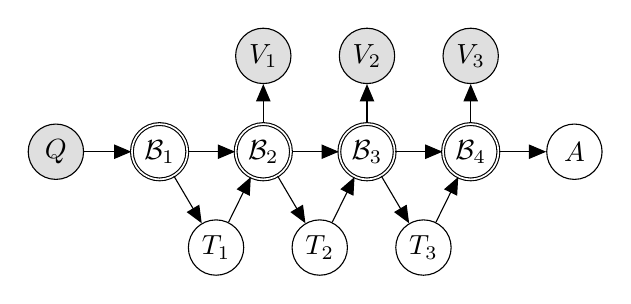
\begin{tikzpicture}
  % Define nodes

  \node[latent]         (T1) {$T_1$};
  \node[latent, right=0.6cm of T1]         (T2) {$T_2$};
  \node[latent, right=0.6cm of T2]         (T3) {$T_3$};
  
%   \node[latent, double, above=0.5cm of Q, xshift=0.6cm]       (stream1) {$\mathcal B_1$};
  \node[latent, double, above=0.5cm of T1, xshift=0.6cm]       (stream2) {$\mathcal B_2$};
  \node[latent, double, left=0.6cm of stream2]       (stream1) {$\mathcal B_1$};
  \node[latent, double, above=0.5cm of T2, xshift=0.6cm]       (stream3) {$\mathcal B_3$};
  \node[latent, double, above=0.5cm of T3, xshift=0.6cm]       (stream4) {$\mathcal B_4$};
%   \node[above=0.5cm of A, xshift=0.6cm]       (stream5) {};

  \node[obs, left=0.6cm of stream1]       (Q) {$Q$};

  
  \node[obs, above=0.5cm of stream2]         (V1) {$V_1$};
  \node[obs, above=0.5cm of stream3]         (V2) {$V_2$};
  \node[obs, above=0.5cm of stream4]         (V3) {$V_3$};

  \node[latent, right=0.6cm of stream4]         (A) {$A$};


  % Connect the nodes
  \edge {Q} {stream1} ; %
  \edge {T1} {stream2} ; %
  \edge {T2} {stream3} ; %
  \edge {T3} {stream4} ; %
  \edge {stream1} {T1} ; %
  \edge {stream2} {T2} ; %
  \edge {stream3} {T3} ; %
  \edge {stream4} {A} ; %
  \edge {stream1} {stream2};
  \edge {stream2} {stream3};
  \edge {stream3} {stream4};
%   \draw [double] (stream1) to (stream2);
%   \draw [double] (stream2) to (stream3);
%   \draw [double] (stream3) to (stream4);
%   \draw [double, ->] (stream4) to (stream5);

%   \edge {stream1} {stream2} ; %
%   \edge {stream2} {stream3} ; %
%   \edge {stream3} {stream4} ; %
%   \edge {stream4} {stream5} ; %
%   \edge {Q} {T1} ; %
%   \edge {T1} {T2} ; %
%   \edge {T2} {T3} ; %
%   \edge {T3} {A} ; %
  \edge {stream2} {V1} ; %
  \edge {stream3} {V2} ; %
  \edge {stream4} {V3} ; %
%   \draw [->] (Q) to [out=-40,in=-140] (A);
%   \path[every node/.style={font=\sffamily\small}]
%     (Q) edge[bend right] node [left] {} (A);
%   \edge[bend right=30] {Q} {A} ; %
\end{tikzpicture}
\caption{Verifier model.
The deterministic $B_t$ nodes are buffer nodes
that accumulate all the past strings.
All other nodes are stochastic.
}
\label{fig:verifier}
\end{figure}








\begin{figure}[h!]
\centering
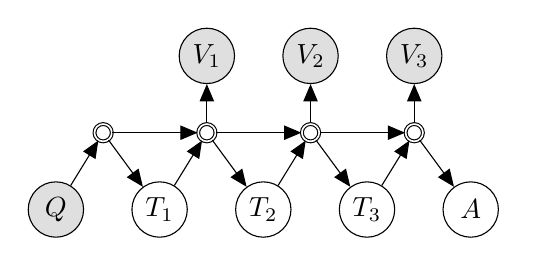
\begin{tikzpicture}
  % Define nodes
  \node[obs]    at (0,0)       (Q) {$Q$};

  \node[latent, right=0.6cm of Q]         (T1) {$T_1$};
  \node[latent, right=0.6cm of T1]         (T2) {$T_2$};
  \node[latent, right=0.6cm of T2]         (T3) {$T_3$};
  \node[latent, right=0.6cm of T3]         (A) {$A$};
  
  \node[latent, double, minimum size=0.22cm, above=0.5cm of Q, xshift=0.6cm]       (stream1) {};
  \node[latent, double, minimum size=0.22cm, above=0.5cm of T1, xshift=0.6cm]       (stream2) {};
  \node[latent, double, minimum size=0.22cm, above=0.5cm of T2, xshift=0.6cm]       (stream3) {};
  \node[latent, double, minimum size=0.22cm, above=0.5cm of T3, xshift=0.6cm]       (stream4) {};
  \node[right=0.4cm of stream4, xshift=0.6cm]       (stream5) {};
  
  \node[obs, above=0.5cm of stream2]         (V1) {$V_1$};
  \node[obs, above=0.5cm of stream3]         (V2) {$V_2$};
  \node[obs, above=0.5cm of stream4]         (V3) {$V_3$};


  % Connect the nodes
  \edge {Q} {stream1} ; %
  \edge {T1} {stream2} ; %
  \edge {T2} {stream3} ; %
  \edge {T3} {stream4} ; %
  \edge {stream1} {T1} ; %
  \edge {stream2} {T2} ; %
  \edge {stream3} {T3} ; %
  \edge {stream4} {A} ; %
%   \draw (stream1) to (stream2);
%   \draw (stream2) to (stream3);
%   \draw (stream3) to (stream4);
%   \draw [double, ->] (stream4) to (stream5);

  \edge {stream1} {stream2};
  \edge {stream2} {stream3};
  \edge {stream3} {stream4};
 % \edge {stream4} {stream5};
 
%   \edge {stream1} {stream2} ; %
%   \edge {stream2} {stream3} ; %
%   \edge {stream3} {stream4} ; %
%   \edge {stream4} {stream5} ; %
%   \edge {Q} {T1} ; %
%   \edge {T1} {T2} ; %
%   \edge {T2} {T3} ; %
%   \edge {T3} {A} ; %
  \edge {stream2} {V1} ; %
  \edge {stream3} {V2} ; %
  \edge {stream4} {V3} ; %
%   \draw [->] (Q) to [out=-40,in=-140] (A);
%   \path[every node/.style={font=\sffamily\small}]
%     (Q) edge[bend right] node [left] {} (A);
%   \edge[bend right=30] {Q} {A} ; %
\end{tikzpicture}
\caption{
Verifier model.
The small double-ringed
nodes are deterministic buffer nodes
that concatenate their inputs, accumulating all past strings.
All other nodes are stochastic. The verifiers are observed to take on the ``correct'' value.
}
\label{fig:verifier}
\end{figure}





We can extend this to  $N$-step reasoning as follows
(where  we drop conditioning on $D$
for brevity):
{\footnotesize
\begin{align*}
p(A|Q,V_{1:N}=1)
&\propto \sum_{T_{1:N}}
p(A,T_{1:N},V_{1:N}=1\,|\,Q),
\end{align*}
}
where
{\footnotesize
\begin{align*}
p(A,T_{1:N},V_{1:N}=1|Q)
&= \left[ \prod_{t=1}^N p(T_t|T_{1:t-1},Q)
p(V_t=1|T_{1:t},Q) \right] \\
& \times p(A|T_{1:N},Q).
\end{align*}
}
\noindent We can represent this 
as shown in \cref{fig:verifier}.
% where the 
% double-ringed nodes are deterministic
% buffer variables that accumulates all the past strings.

% TODO: Clarify this. bpoole didn't get & he understands ladder VAEs well
%(This restores the first-order Markov property,
%and is similar to how RNNs are used
%to define ladder VAEs \citep{Sonderby2016ladder}.)

To see why such a verification model can be useful,
consider (for simplicity) the case where $N=1$.
Suppose we have trained the model to generate valid
thoughts and answers by giving it suitable training examples,
and then we generate $K$ samples
$(T^k,V^k,A^k) \sim p(T,V,A|Q,D)$.
We can then rank the samples for validity by computing
$r^k = p(V^k=1|A^k, Q, D)$,
and then picking the  $A^k$ with largest score $r^k$.

\citet{verifiers} train the verifier to predict a binary correctness label.  \citet{language_feedback} incorporates natural language feedback, and finds that learning is significantly more sample efficient. Preliminary evidence suggests that LMs are capable of critiquing their own chain of reasoning in language, in which case the verifier produces natural language and $p(V_{1:N} = 1 | Q, A, T_{1:N})$ becomes the likelihood of the verifier taking on a particular string value, such as $p(V_{1:N}=\text{"The reasoning and solution are correct."} | ...)$. \citet{openai_critique} study model generated critiques in the context of summarization.

% \ddohan{We view this feedback as an auxiliary variable which can be conditioned to inform inference.}

% \kevin{Should we mention Rapha's preliminary results?}

\begin{comment}
One way to perform inference in this model 
would be to use
particle filtering. The hope is that, by conditioning
on $V_{1:N}=1$,
we increase the probability that the sampled
$T_{1:N}$ values constitute
a valid chain of reasoning
for deriving $A$ from $Q$ and $D$.
This can then provide higher quality training data
in an EM-like fine-tuning scheme, similar
to STaR in \cref{sec:STAR}.
However, we leave evaluation of this idea to future work.
\end{comment}

\subsection{Tool-use}
The applications discussed so far involve iterating a language model, within some control flow, without external feedback. There are many tasks of interest in which a model is interacting with external systems. \citet{verifiers} has an LM use a calculator to solve math tasks, while \citet{webgpt} put an LM in a loop with a web browser to answer questions. Using PPLs to represent these probabilistic models allows easily representing these cases, by writing the call to the external tool, such as the calculator, directly
into the program.
Then techniques from simulation based inference, for example, can be applied to do inference in such situations \cite{simulation_inference}.

\begin{comment}
\charles{Suggest cut for time.}
\kevin{Agreed}
%\begin{tikzpicture}
%  % Define nodes
%  \node[obs]           (Q) {$Q$};
%  \node[latent, right=0.6cm of Q]         (act_1) {$\text{action}_1$};
%  \node[latent, right=0.6cm of Q]         (act_2) {$\text{action}_{...}$};
%  \node[latent, right=0.6cm of Q]         (act_3) {$\text{action}_n$};
%  
%  \node[latent, rectangle]           (env1) {$env_1$};
%  \node[latent, rectangle]           (env2) {$env_2$};
%  \node[latent, rectangle]           (env3) {$env_3$};
%
%  % Connect the nodes
%  %\edge {Q} {T} ; %
%  %\edge {T} {A} ; %
%  %\draw [->] (Q) to [out=40,in=140] (A);
%%   \path[every node/.style={font=\sffamily\small}]
%%     (Q) edge[bend right] node [left] {} (A);
%%   \edge[bend right=30] {Q} {A} ; %
%\end{tikzpicture}
%
\end{comment}
\subsection{Twenty questions}
\label{sec:twenty}

In this section, we discuss experimental results using \cascades\ to solve the
 ``Twenty Questions'' task from BigBench \citep{bigbench}.
This task  involves a conversation between two agents, Alice and Bob.
Both agents are presented with the rules of the game, and Alice is additionally presented with a concept (e.g. `apple') to describe.
Bob has to guess the concept by asking a series of  questions
$B_t$ of the form ``Is it X?'', to which Alice answers
$A_t \in \{ \text{`Yes.'}, \text{`No.'}\}$.
We repeat this process until Bob guesses correctly, or we hit the limit of $T$ rounds.
This can be thought of as a pair of interacting Markov chains, which exchange strings, until some final end state is reached,
 as illustrated in \cref{fig:twenty}.


\begin{figure}[h!]
\centering
% \begin{tikzpicture}
%   % Define nodes
%   \node[obs]    at (0,0)       (C) {\tiny{\texttt{CONCEPT}}};
%   \node[latent, right=1.4cm of C]         (A1) {$A_1$};
%   \node[latent, right=0.9cm of A1]         (A2) {$A_2$};
% %   \node[latent, right=0.6cm of A2]         (A3) {$A_3$};
%   \node[latent, above=0.6cm of A1, xshift=-.8cm]         (B1) {$B_1$};
%   \node[latent, right=0.9cm of B1]         (B2) {$B_2$};
% %   \node[latent, right=0.6cm of B2]         (B3) {$B_3$};

%   \node[obs, left=0.75cm of B1]           (R) {\tiny{\texttt{RULES}}};

%   \node[right=0.3cm of B2] (label1) {\Large\textbf{. . .}};
%   \node[right=0.3cm of A2] (label1) {\Large\textbf{. . .}};


%   % Connect the nodes
%   \edge {R} {B1} ; %
%   \edge {C,R,B1} {A1} ; %
%   \edge {R,A1,B1,B2} {A2} ; %
% %   \edge {A2,B2,B3} {A3} ; %
%   \edge {R} {B1} ; %
%   \edge {A1,B1} {B2} ; %
% %   \edge {A2,B2} {B3} ; %
%   \draw [->] (R) to [out=40,in=140] (B2);
%   \draw [->] (C) to [out=-40,in=-140] (A2);
% %   \draw [->] (Q) to [out=40,in=140] (A);
% %   \draw [->] (S) to [out=40,in=140] (A);
% \end{tikzpicture}

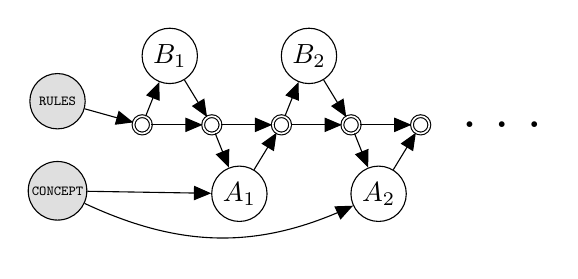
\begin{tikzpicture}
  \node[obs]       (R) {\tiny{\texttt{RULES}}};

  \node[obs, below=0.4cm of R]       (C) {\tiny{\texttt{CONCEPT}}};

% stream
  \node[latent, double, minimum size=0.22cm, right=0.6cm of R, yshift=-0.3cm]       (BS1) {};
  \node[latent, double, minimum size=0.22cm, right=0.65cm of BS1]       (BS2) {};
  \node[latent, double, minimum size=0.22cm, right=0.65cm of BS2]       (BS3) {};
  \node[latent, double, minimum size=0.22cm, right=0.65cm of BS3]       (BS4) {};
  \node[latent, double, minimum size=0.22cm, right=0.65cm of BS4]       (BS5) {};

  \node[latent, above=0.4cm of BS1, xshift=0.35cm]         (B1) {$B_1$};
  \node[latent, above=0.4cm of BS3, xshift=0.35cm]         (B2) {$B_2$};
%   \node[latent, right=0.9cm of B1]         (B2) {$B_2$};

  \node[latent, below=0.4cm of BS2, xshift=0.35cm]         (A1) {$A_1$};
  \node[latent, below=0.4cm of BS4, xshift=0.35cm]         (A2) {$A_2$};


  \node[right=0.3cm of BS5] (label1) {\Large\textbf{. . .}};

    \edge {R} {BS1} ; 
    \edge {BS1} {BS2}; 
    \edge {BS2} {BS3}; 
    \edge {BS3} {BS4}; 
    \edge {BS4} {BS5}; 

    \edge {BS1} {B1} ;
    \edge {B1} {BS2} ;
    \edge {BS2} {A1} ;
    \edge {A1} {BS3} ;
    \edge {BS3} {B2} ;
    \edge {B2} {BS4} ;
    \edge {BS4} {A2} ;
    \edge {A2} {BS5} ;

    \edge {C} {A1} ;
      \draw [->] (C) to [out=-25,in=-155] (A2);


\end{tikzpicture}

% \begin{tikzpicture}

%   \node[obs]    at (0,0)       (C) {\tiny{\texttt{CONCEPT}}};
%   \node[obs, above=0.3cm of C]           (R) {\tiny{\texttt{RULES}}};

% %% alice stream
%   \node[latent, double, minimum size=0.22cm, right=0.6cm of C, yshift=0.15cm]       (AS1) {};
%   \node[latent, double, minimum size=0.22cm, right=0.65cm of AS1]       (AS2) {};
%   \node[latent, double, minimum size=0.22cm, right=0.65cm of AS2]       (AS3) {};
%   \node[latent, double, minimum size=0.22cm, right=0.65cm of AS3]       (AS4) {};
%   \node[latent, double, minimum size=0.22cm, right=0.65cm of AS4]       (AS5) {};

% %% bob stream
%   \node[latent, double, minimum size=0.22cm, above=0.6cm of AS1]       (BS1) {};
%   \node[latent, double, minimum size=0.22cm, right=0.65cm of BS1]       (BS2) {};
%   \node[latent, double, minimum size=0.22cm, right=0.65cm of BS2]       (BS3) {};
%   \node[latent, double, minimum size=0.22cm, right=0.65cm of BS3]       (BS4) {};
%   \node[latent, double, minimum size=0.22cm, right=0.65cm of BS4]       (BS5) {};

%   \node[latent, above=0.4cm of BS1, xshift=0.3cm]         (B1) {$B_1$};
%   \node[latent, right=0.9cm of B1]         (B2) {$B_2$};

%   \node[latent, below=.4cm of AS2, xshift=0.3cm]         (A1) {$A_1$};
%   \node[latent, right=0.9cm of A1]         (A2) {$A_2$};

%     \edge {BS1} {B1} ;
%     \edge {B1} {BS2,AS2}

%     \edge {C,R} {AS1} ; 
%     \edge {AS1} {AS2}; 
%     \edge {AS2} {AS3}; 
%     \edge {AS3} {AS4}; 
%     \edge {AS4} {AS5}; 
%     \edge {R} {BS1} ; 
%     \edge {BS1} {BS2}; 
%     \edge {BS2} {BS3}; 
%     \edge {BS3} {BS4}; 
%     \edge {BS4} {BS5}; 


% \end{tikzpicture}



\caption{Twenty questions.}
\label{fig:twenty}
\end{figure}


% \begin{align*}
% \text{question}, \text{facts} \ &\sim \text{Tasks} \\
% \text{selection} &\sim S(\text{question}, \text{facts}) \\
% \text{inference} &\sim S(\text{question}, \text{selection}) \\
% \text{answer} &\sim S(\text{question}, \text{inference}) \\
% \text{reward} &\sim \text{Judge}(\text{answer}, \text{question})
% \end{align*}

The goal is to infer what questions Bob should ask to guess the concept as quickly as possible. This can be cast as a reinforcement learning problem with string-valued actions, or equivalently as an inference problem where we condition on the goal state that $A_T=\text{`yes'}$ for the soonest possible $T$ (c.f., planning as inference \cite{rl_inference}). %\todo{JSD: This is inaccurate -- Alice's answers can be yes or no for any question, regardless of whether Bob correctly guessed the concept.}.
%, goal-conditioned policies such as decision-transformer \cite{decision_transformer} and upside-down RL \cite{upsidedown_rl})

In our current preliminary experiments, we use a forward sampling
approach (aka ancestral sampling), in which 
we sample 50 conversations per concept with temperature $1.0$.
We consider a trial successful if the target concept appears in $B_t$.
(i.e., Bob guesses the right answer).
We reject a sampling chain early if it is ``malformed''
(e.g., Bob generates a response that is not a question).

%at least one of these samples has
% $A_t=\text{`yes'}$ for some $t \leq T$
%[JSD: I think this should rather be that we accept the chain if the concept being communicated appears in $B_t$? $A_t$ can be yes or no for any question.]

% TODO: Add this back in after deanonymized
%We use the pretrained "Lamda" LLM with 137B parameters \cite{lamda}.

Bob's turn starts with `Is the concept' which we complete with the LM. Then we let Alice generate an answer;
we post-process Alice's response
by replacing all mentions of the 
true concept with the generic  word ``concept", to prevent information leakage. 
%\rif{Why not use rejection sampling to constrain Alice to answer yes or no, which we said was the rule?} We repeat this for 10 rounds.
%\ddohan{We should have - no good reason.}
Using the LaMDA 137B large LM \citep{lamda},
we find that the model is able to solve $29\%$ of the tasks. %\rif{Is that good?}
See Appendix~\ref{app:20q-details} for more details.

% \section{Scope and limitations}
% We frame many existing algorithms for composing models in terms of probabilistic programming. While this suggests the possibility of applying a variety of existing inference and train-time techniques to the resulting models, the present work does not evaluate methods beyond rejection sampling.
% 
% A challenge applying cascades in practice is the difficulty of probabilistic inference in models with string-valued variables. Previous work in particle based inference for probabilistic programs provides some hope in this direction \citep{anglican}.

% This perspective opens up exciting new directions in applications of language models, and in foundation models more generally.
% Existing fine-tuning methods can be described with a principled probabilistic programming language formalism representing structured distributions known as LM Cascades. This defines the distribution on the string-valued output of a large language model, the compositions of which may be adapted as specific inference algorithms underpinning various applications. 


% efficiency / expense
% We don't actually explore specific inference methods
% Hint of 
% hints @ lots of possibilities, explores very few of them
% - multimodality
% - train/test time inference beyond rejection sampling
% - tool use
%\section{Conclusion and future work}
\section{Discussion}
% TODO: Combine conclusion, limitations, and future work
We have shown how probabilistic programming provides a flexible formalism for composing models together to define complex probabilistic models over strings, placing many existing algorithms in a unified framework. While this suggests the possibility of applying a variety of existing inference and train-time techniques to the resulting models, the present work does not evaluate methods beyond rejection sampling.

%beyond the examples that we mentioned, one can also use this framework
%to represent lms that interact with external systems,
%such as calculators or search engines,
%in order to perform a variety of tasks.
We can also cast many planning and RL tasks in our framework, by using the perspective of control as inference.
While we restrict presentation to the string setting, the ideas presented here are applicable to multimodal settings as well, allowing us to combine image and text models into a larger system.

% We frame many existing algorithms for composing models in terms of probabilistic programming. While this suggests the possibility of applying a variety of existing inference and train-time techniques to the resulting models, the present work does not evaluate methods beyond rejection sampling.
A challenge applying cascades in practice is the difficulty of probabilistic inference in models with string-valued variables. Previous work in particle based inference for probabilistic programs provides some hope in this direction \citep{anglican}.

The core technical challenge is efficient inference, 
as is usually the case with PPLs. A key insight, which we intend
to explore in future work, is that we can emulate posterior
inference by training the LM 
to ``fill in the blanks'', corresponding to the unknown variables.
A similar idea is explored in 
foundation posteriors \citep{foundationposterior}, applied to Stan probabilistic programs, demonstrating that LMs are applicable to numerical data types as well.
In other words, we can use LMs as proposal distributions,
or guide networks.
%as well as a way of specifying the model.
We also intend to explore fine-tuning methods, going
beyond the few-shot prompting approach described here.

Recent advances in program synthesis suggest the possibility of \textit{probabilistic program induction} \citep{Lake2015,language_of_thought} to search for \cascades which solve a target task, rather than assuming a fixed probabilistic program structure.


% !TEX root = main.tex

\section*{Acknowledgments}

\vspace*{-1ex}

The authors would like to thank Kyunghyun Cho and Thomas Fuchs for helpful discussions, Joost Huizinga, Anh Nguyen, and Roby Velez for editing, as well as funding from 
the NASA Space Technology Research Fellowship (JY), DARPA project W911NF-12-1-0449, NSERC, Ubisoft, and CIFAR
(YB is a CIFAR Fellow).


\bibliography{paper}
\bibliographystyle{icml2022}


\newpage
\appendix
\onecolumn
\appendix

% \section{Claimed Emergent Abilities}
% \label{app:claimed_emergent_abilities}

% We compile the models, tasks and metrics that different papers have claimed reveal emergent abilities of large language models. This list may be incomplete or inaccurate, but represents a good faith attempt to compile this information. Note: quantifying model scale when an ability emerges is complicated by the fact that different papers report model scale differently, either as (a) number of parameters \cite{brown2020language, ganguli2022predictability}, (b) effective number of parameters \cite{srivastava2022beyond} or (c) training FLOPs \cite{wei2022emergent}.

% \begin{table}[h!]
%     \centering
%     \begin{tabular}{|l|c|c|c|}
%     \hline
%         Task & Model Families & Metric & Model Scale at Emergence \\
%         \hline
%         2-Digit Addition \cite{brown2020language} & GPT-3 & Accuracy & 13B Parameters\\
%         2-Digit Subtraction \cite{brown2020language} & GPT-3 & Accuracy & 13B Parameters\\
%         3-Digit Addition \cite{brown2020language, ganguli2022predictability} & GPT-3 & Accuracy & 175B Parameters\\
%         3-Digit Subtraction \cite{brown2020language} & GPT-3 & Accuracy & 175B Parameters\\
%         MMLU \cite{ganguli2022predictability} & GPT-3, Gopher & Accuracy & 200B, 300B Parameters\\
%         Program Synthesis \cite{ganguli2022predictability} & Google Internal & \% Samples Solving Task & 200B Parameters\\
%         Figure of Speech Detection \cite{srivastava2022beyond} & ? & ? & $\sim 10^{11}$ Effective Parameters \\
%         IPA Transliterate \cite{srivastava2022beyond, wei2022emergent} & LaMDA, GPT-3 & BLEU & $\sim 10^{23}, \sim 10^{23}$ Training FLOPs\\
%         Periodic Elements \cite{srivastava2022beyond} & ? & ? & ?\\
%         Modified Arithmetic \cite{srivastava2022beyond, wei2022emergent} & GPT-3, LaMDA & Accuracy & $\sim 10^{23}, \sim 10^{24}$ Training FLOPs\\
%         Repeat Copy Logic \cite{srivastava2022beyond} & ? & ? & $10^{11}$ Effective Parameters\\
%         Word Unscrambling \cite{srivastava2022beyond, wei2022emergent} & LaMDA & Exact Match & $\sim 10^{24}$ Training FLOPs\\
%         Persian QA \cite{wei2022emergent} & PaLM & Exact Match & $\sim 10^{24}$ Training FLOPs\\
%         Truthful QA \cite{wei2022emergent} & Gopher & Accuracy & $\sim 10^{23}$ Training FLOPs\\
%         Grounded Mappings \cite{wei2022emergent} & ? & ? & ?\\
%         Multi-task NLU \cite{wei2022emergent} & ? & ? & ?\\
%         Word in context \cite{wei2022emergent} & ? & ? & $\sim 10^{24}$ Training FLOPs\\
%         \hline
%     \end{tabular}
%     \newline
%     \caption{\textbf{Tasks, model families, metrics and number of parameters for emergent abilities.}}
%     \label{tab:my_label}
% \end{table}


% \section{Exponentiated Negative Cross Entropy Lower Bounds Accuracy}
% \label{app:acc_bound}

% Consider batch size $B$ with length $L$. During training i.e. with teacher-forcing, the per-token accuracy (averaged over batch index $b$ and sequence index $l$) is defined as:
% %
% \begin{align}
%     \text{Acc} &\defeq \frac{1}{B} \sum_b \frac{1}{L} \sum_l p(t_{bl}^* | t_{b, <l}^*)\\
%     &= \frac{1}{BL} \sum_{b, l} p(t_{bl}^* | t_{b, <l}^*)
% \end{align}

% The cross entropy (commonly averaged over the batch) is defined as:
% %
% \begin{align}
%     \mathcal{L}_{CE} &\defeq -\frac{1}{B} \sum_b \log p(t_{b 1}^*, ..., t_{b L}^*)\\
%     &= -\frac{1}{B} \sum_b \log \prod_l p(t_{b l}^*| t_{b, <l}^*)\\
%     &= -\frac{1}{B} \sum_{b, l} \log p(t_{bl}^* | t_{b, <l}^*)
% \end{align}

% To make the comparison between accuracy and cross entropy a little easier, let's normalize the cross entropy by the sequence length:
% %
% \begin{align}
%     \mathcal{L}_{CE/L} &\defeq \frac{1}{L}\mathcal{L}_{CE}\\
%     &=  -\frac{1}{BL} \sum_{b, l} \log p(t_{bl}^* | t_{b, <l}^*)
% \end{align}

% Recall that Jensen's inequality tells us that for any random variable $X$, $\log \mathbb{E}[X] \geq \mathbb{E}[\log X]$. The relationship between sequence-length-normalized cross entropy and accuracy is thus:
% %
% \begin{align}
%     -\mathcal{L}_{CE/L} = \frac{1}{BL} \sum_{b, l} \log p(t_{bl}^* | t_{b <l}^*) &\leq \log \frac{1}{BL} \sum_{b, l}  p(t_{bl}^* | t_{b <l}^*) = \log \text{Acc}\\
%     \exp(- \mathcal{L}_{CE/L}) &\leq \text{Acc}
% \end{align}

% Consequently, we see that driving the cross entropy loss to $0$ necessarily drives the accuracy to $1$.

% TODO: Can we use the second moment method to derive bounds on how (un)likely a subset of tokens are to deviate from the mean?


\section{Approximate Behavior of Metrics on Sequential Data}
\label{app:metric_scaling}

How do different metrics behave when used to measure autoregressive model outputs? Precisely answering this question is tricky and possibly analytically unsolvable, so we provide an approximate answer here.

Notationally, we consider $N$ test data of length $L$ (here, length is measured in tokens) with targets denoted $t_n \defeq (t_{n1}, t_{n2}, ... t_{nL})$, the autoregressive model has a true-but-unknown per-token error probability of $\epsilon \in [0, 1]$ and the model outputs prediction $\hat{t}_n \defeq (\hat{t}_{n1}, \hat{t}_{n2}, ... \hat{t}_{nL})$. This assumes that the model's per-token error probability is constant, which is empirically false, but modeling the complex dependencies of errors is beyond our scope.

\subsection{Per-Token Error Probability is Resolution-Limited}
\label{app:metric_scaling:resolution_limited}

Note that because we have $N$ test data, each of length $L$, our resolution for viewing the per-token error probability $\epsilon$ is limited by $1/NL$. 
Here, resolution refers to ``the smallest interval measurable by a scientific instrument; the resolving power."
To explain what resolution means via an example, suppose one wants to measure a coin's probability of yielding heads.
After a single coin flip, only two outcomes are possible (H, T), so the resolution-limited probability of heads is either $0$ or $1$.
After two coin flips, four outcomes are possible (HH, HT, TH, TT), so the resolution-limited probability of heads is now one of $0, 0.5, 1$.
After $F$ coin flips, we can only resolve the coin's probability of yielding heads up to $1/F$.
Consequently, we introduce a resolution-limited notation:
%
\begin{equation}
    \nint{a}_b \defeq \text{$a$ rounded to the nearest integer multiple of $1/b$}
\end{equation}

\subsection{Token Edit Distance}
\label{app:metric_scaling:token_edit_distance}

We first consider an adaptation of the Levenshtein (string edit) distance for models that function on tokens rather than characters, an adaptation we term the \textit{token edit distance}. The token edit distance between two token sequences $t_n, \hat{t_n}$ is defined as the integer number of additions, deletions or substitutions necessary to transform $t_n$ into $\hat{t}_n$ (or vice versa).

\begin{align}
    \text{Token Edit Distance}(t_n, \hat{t}_n)  &\defeq \text{Num Substitutions} + \text{Num. Additions} + \text{Num. Deletions}\\
    &= \sum_{\ell =1}^L \mathbb{I}[t_{n\ell} \neq \hat{t}_{n\ell}] + \text{Num. Additions} + \text{Num. Deletions}\\
    &\geq \sum_{\ell =1}^L \mathbb{I}[t_{n\ell} \neq \hat{t}_{n\ell}]
\end{align}

The expected token edit distance is therefore:

\begin{align}
    \mathbb{E}[\text{Token Edit Distance}(t_n, \hat{t}_n)] &\geq \mathbb{E}[\sum_{\ell =1}^L \mathbb{I}[t_{n\ell} \neq \hat{t}_{n\ell}]]\\
    &= \sum_{\ell =1}^L p(t_{n\ell} \neq \hat{t}_{n\ell})\\
    &\approx L (1 - \epsilon)
\end{align}

The resolution-limited expected token edit distance is therefore:

\begin{equation}
    \nint{\mathbb{E}[\text{Token Edit Distance}(t_n, \hat{t}_n)]}_{NL} \geq L \Big(1 - \nint{\epsilon}_{NL} \Big)
\end{equation}

From this, we see that the expected token edit distance scales approximately linearly with the resolution-limited per-token probability. The real rate is slightly higher than linear because additions and deletions contribute an additional non-negative cost, but modeling this requires a model of how likely the model is to overproduce or underproduce tokens, which is something we do not currently possess.

\subsection{Accuracy}
\label{app:metric_scaling:accuracy}

\begin{align}
    \text{Accuracy}(t_n, \hat{t}_n) &\defeq \mathbb{I}[\text{No additions}] \, \mathbb{I}[\text{No deletions}] \, \prod_{l=1}^L \mathbb{I}[t_{nl} = \hat{t}_{nl}]\\
    &\approx \prod_{l=1}^L \mathbb{I}[t_{nl} = \hat{t}_{nl}]
\end{align}

As with the Token Edit Distance (App. \ref{app:metric_scaling:accuracy}), we ignore how likely the language model is to overproduce or underproduce tokens because we do not have a good model of this process. Continuing along,

\begin{align}
    \mathbb{E}[\log \text{Accuracy}] &= \sum_l \mathbb{E}[\log \mathbb{I}[t_{nl} = \hat{t}_{nl}]]\\
    &\leq \sum_l \log \mathbb{E}[\mathbb{I}[t_{nl} = \hat{t}_{nl}]]\\
    &\approx L \log (1- \epsilon)
    % \exp(\mathbb{E}[\log \text{Accuracy}]) &= \exp (\sum_l \mathbb{E}[\log \mathbb{I}(t_{nl}, \hat{t}_{nl})])\\
    % &=
\end{align}

Taking an approximation that would make most mathematicians cry:

\begin{align}
    \mathbb{E}[\text{Accuracy}] &\approx \exp(\mathbb{E}[\log \text{Accuracy}])\\
    &= (1 - \epsilon)^L\\
\end{align}

This reveals that accuracy \textbf{approximately} falls geometrically with target token length. The resolution-limited expected accuracy is therefore:

\begin{equation}
    \nint{\mathbb{E}[\text{Accuracy}]}_{NL} = \nint{(1 - \epsilon)^L}_{NL}
\end{equation}

From this we can see that choosing a nonlinear metric like Accuracy is affected significantly more by limited resolution because Accuracy forces one to distinguish quantities that decay rapidly.

\subsection{ROUGE-L-Sum}
\label{app:metric_scaling:rougeLsum}

\begin{figure}
    \centering
    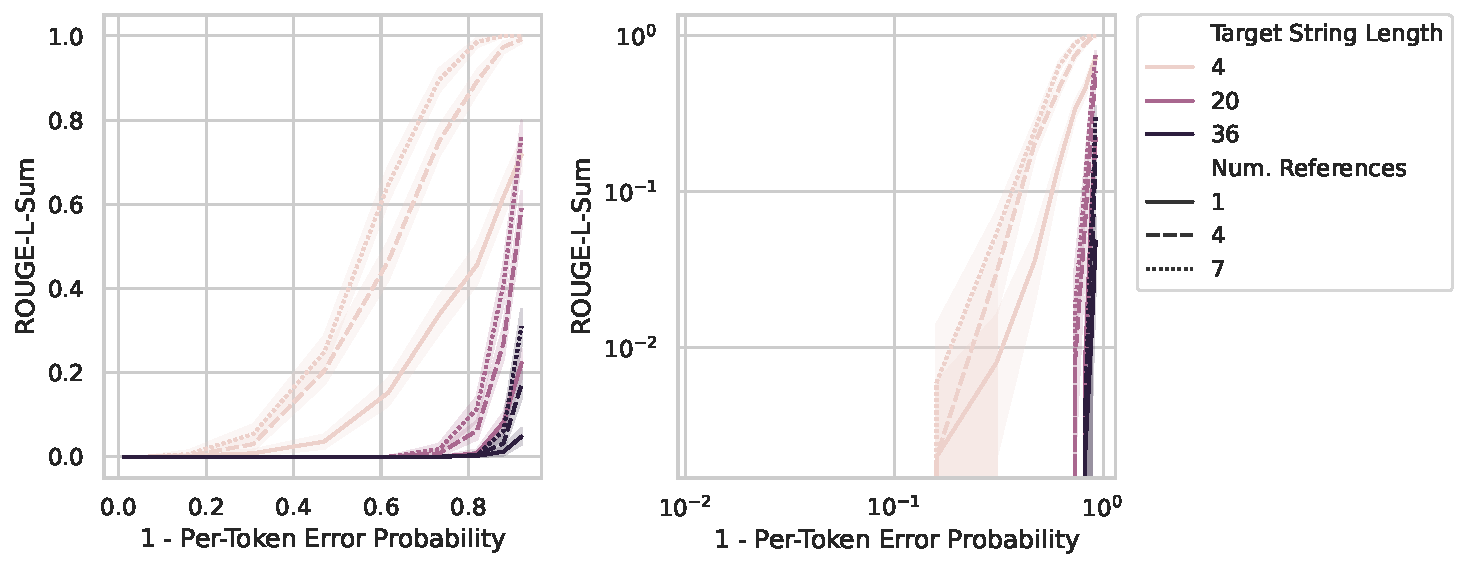
\includegraphics[width=0.95\textwidth]{figures/rouge_understanding/rougeLsum_vs_token_error_prob_scaling_simulation.pdf}
    \caption{\textbf{ROUGE-L-Sum is a sharp metric.} Simulations show that as the per-token error probability slightly increase (e.g. from 0.05 to 0.1), the ROUGE-L-Sum metric sharply falls.}
    \label{fig:app:metric_scaling:rougeLsum}
\end{figure}


Another BIG-Bench metric \cite{srivastava2022beyond} is ROUGE-L-Sum \cite{lin2004rouge}, a metric based on the longest common subsequence (LCS) between two sequences. Section 3.2 of \cite{lin2004rouge} gives the exact definition, but the key property is that ROUGE-L-Sum measures the ``union" LCS, which means ``stitching" together LCSs across the candidate and multiple references. As explained in the original paper: if the candidate sequence is $c = w_1 w_2 w_3 w_4 w_5$, and if there are two reference sequences $r_1 = w_1 w_2 w_6 w_7 w_8$ and $r_2 = w_1 w_3 w_8 w_9 w_5$, then $LCS(r_1, c) = w_1 w_2$ and $LCS(r_2, c) =w_1 w_3 w_5$, then the \textit{union} 
-LCS of $c, r_1, r_2$ is $w_1 w_2 w_3 w_5$, with length 4. Intuitively, this disproportionately benefits models with smaller error rates because their mistakes can be ``stitched" across multiple references; this is confirmed in simulation (Fig. \ref{fig:app:metric_scaling:rougeLsum}).


% \subsection{BLEU}
% \label{app:metric_scaling:bleu}


% \subsection{Emergence does not require on scaling laws: decreasing cross-entropy loss and stricter exact match is all you need }

% The goal of this section is to show that scaling laws are not necessary to create emergence and that many functional forms of the loss are valid as long as the form decreases as some other variable decreases -- say the number of parameters in the model.
% This typically holds in modern machine learning. 
% We do this by considering different functional forms of the cross entropy $CE(N)$, as a function of the number of parameters $N$, and show emergence, i.e. sharpness and unpredictability.
% We illustrate this by showing the programmer can exaggerate the sharpness (and therefore emergence) by implying increasing the exact number of tokens required to get correct in the accuracy, i.e. increasing $L$ in our notation.

% \subsubsection{Argument}

% Recall from section \ref{sec:alt_explanation} the accuracy requiring all $L$ tokens to be correct for a model of size $N$ as a function of cross-entropy $CE(N)$:

% \begin{equation*}
%     \text{Accuracy}(N) \approx p_N(\text{single token correct})^{\text{num. of tokens}} = \exp \Big(- CE(N) \Big)^L
% \end{equation*}

% We plot this equation using three functional forms for a decreasing cross-entropy loss in figure \ref{fig:decreasing_loss_leads_to_emergence_as_L_increases} for increasing values of $L$.
% These increasing values of $L$ induce a sharper -- therefore, seemingly more emergent curve when plotting the accuracy. 
% This means that if the programmer simply requires a stricter accuracy, he can make a perfectly smooth and predictable cross-entropy loss suddenly become sharp and unpredictable, i.e. ``emergent". 
% We show numerically it is independent of the functional form and instead that it only requires the cross-entropy to be decreasing and the accuracy metric to have some non-linear transformation that makes it sharper. 
% Therefore, if one had only tracked the cross-entropy loss instead, one could have had a smooth predictable curve for the models.
% This implies small-scale experimentation is still relevant, and we wish to highly that GPT-4 \cite{gpt4} small-scale experiment in conjunction with scaling loss. 
% We'd like to emphasize that changing the evaluation metric can suddenly induce emergence, and it is not an intrinsic property of the model. 

% %The goal will be to show that if $CE(N)$ decreases with different functional forms that $acc$ is emergent (either sharp or unpredictable).
% % TODO: sharp due to L
% % TODO: unpredictable due to constant and L

% \begin{figure}[htbp]
%   \centering
%   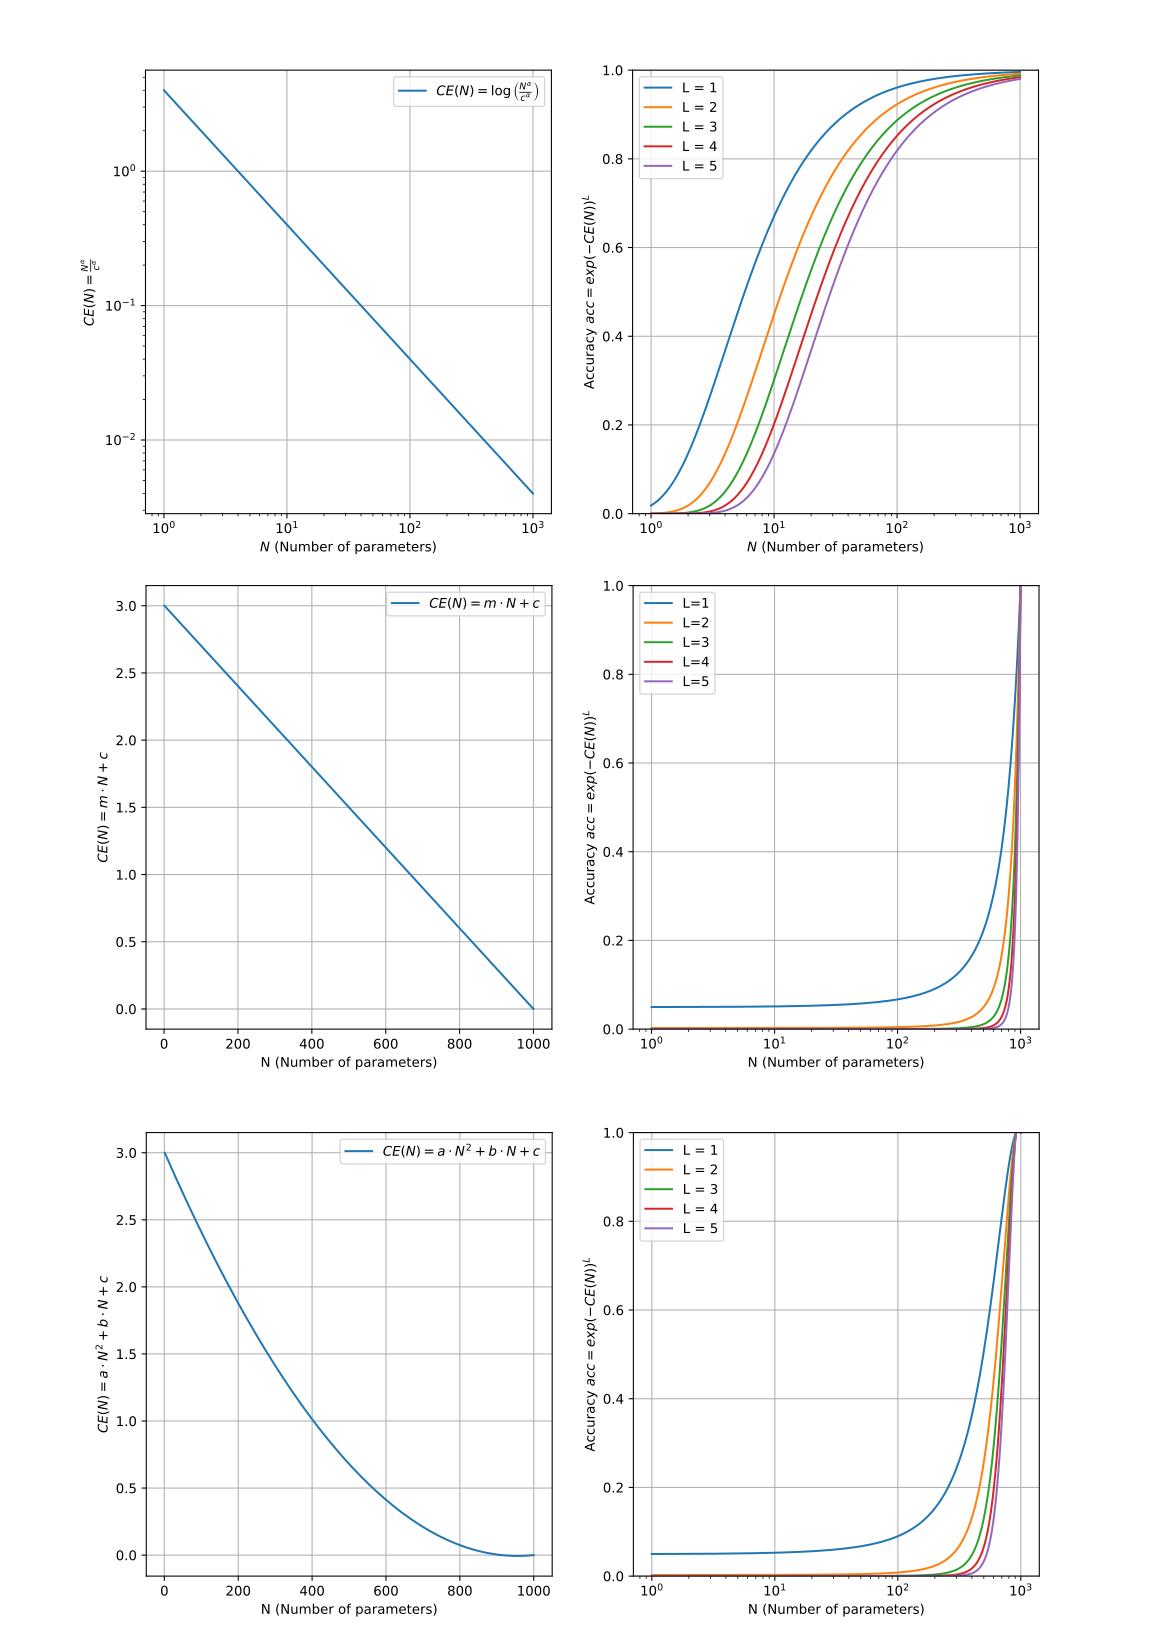
\includegraphics[width=0.8\textwidth]{figures/loss_decreasing_leads_to_emergence/decreasing_loss_leads_to_emergence_as_L_increases.png}
%   \caption{
%   \textbf{Emergence does not depend on scaling laws: any decreasing cross-entropy loss induces apparent emergence as L increases as you require more tokens to be exactly correct, i.e. L increases.}
%   The first row shows the same argument as in the main section, where a decreasing cross-entropy loss as a scaling law induces emergence as $L$ increases.
%   The second row shows the that apparent emergence is induced even when the cross-entropy loss decreases linearly.
%   The third row shows that the apparent emergence is induced when the cross-entropy loss decreases quadratically.
%   Emergence is amplified in this case especially by the increase in sharpness as more tokens are required to be correct. 
%   This means that simply changing the evaluation metric can suddenly induce emergence, and it is not an intrinsic property of the model. 
%   }
%   \label{fig:decreasing_loss_leads_to_emergence_as_L_increases}
% \end{figure}


\section{Inducing Emergent Abilities in Networks on Vision Tasks}
\label{app:sec:inducing_emergence_vision}

\subsection{Emergent Classification of MNIST Handwritten Digits by Convolutional Networks}

\begin{figure}
    \centering
    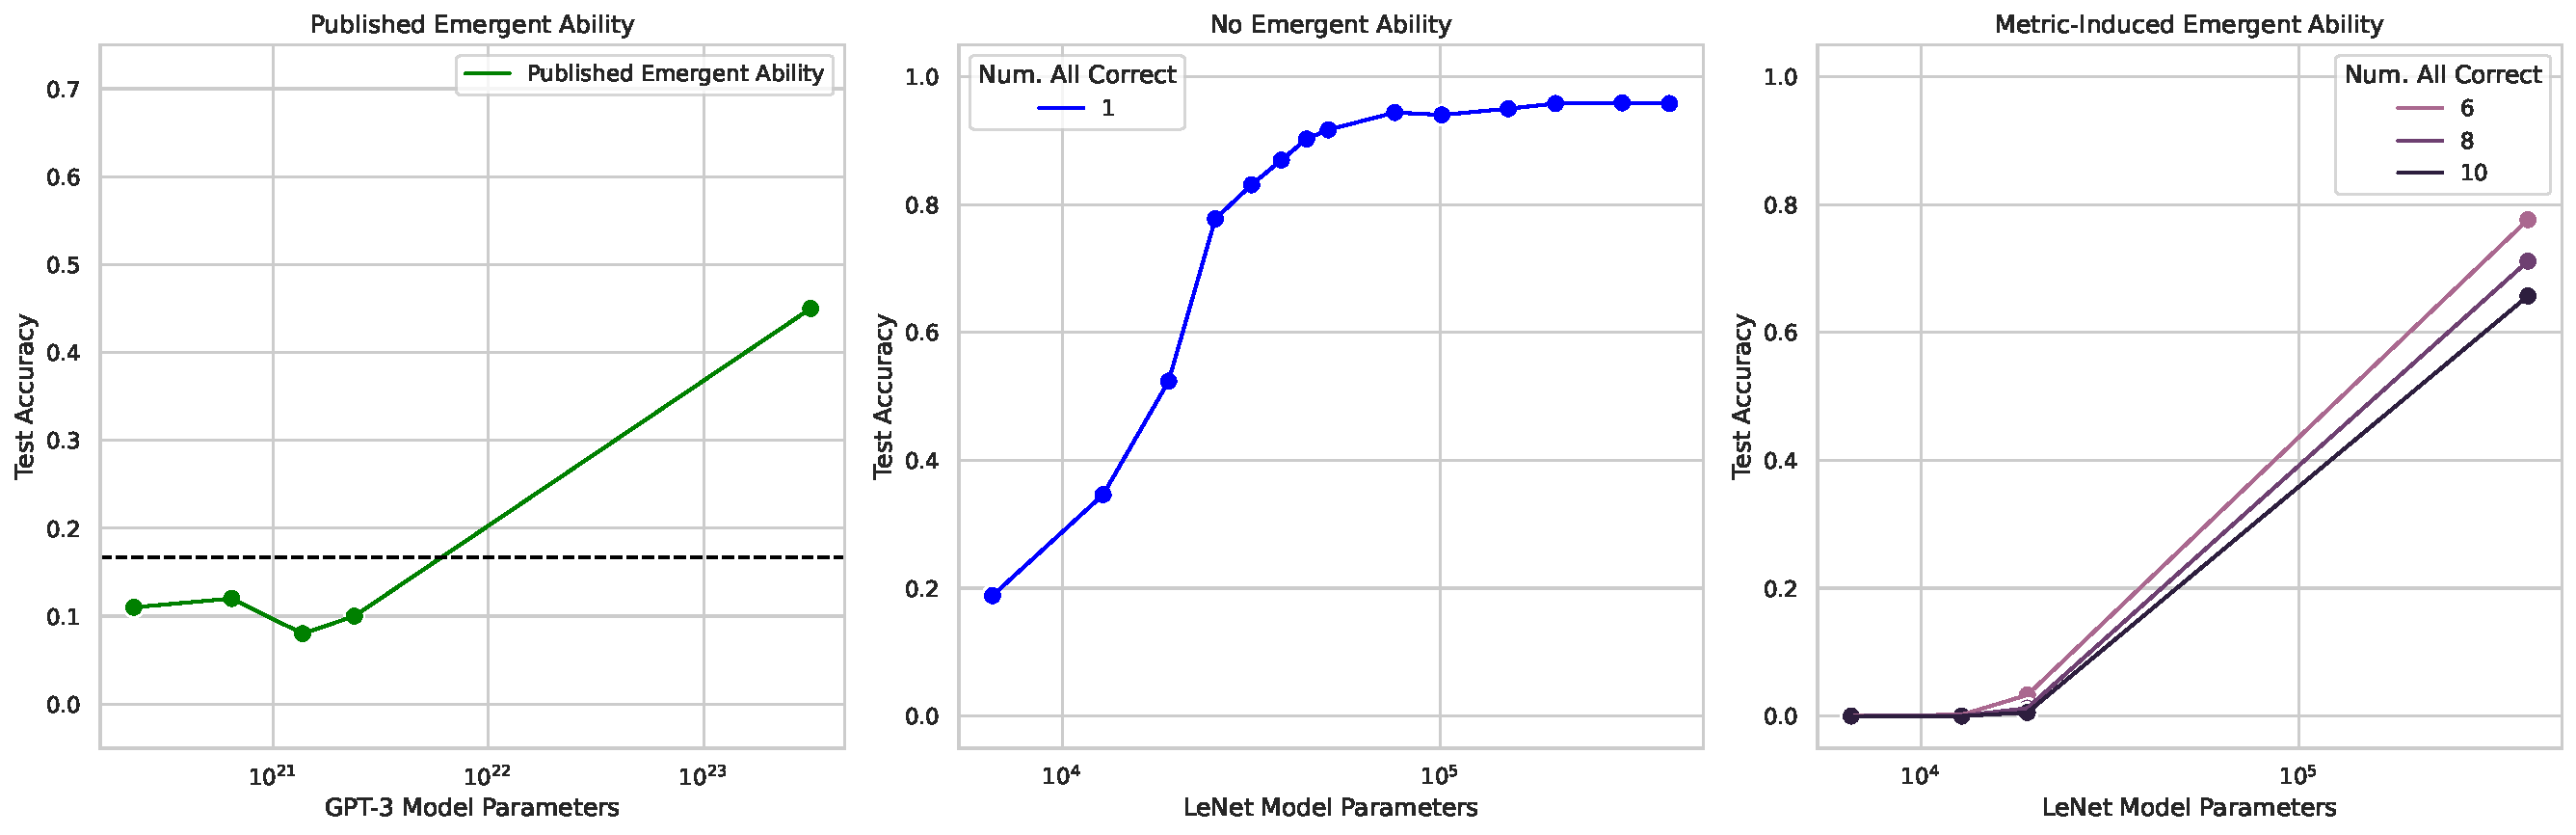
\includegraphics[width=\textwidth]{figures/vision/no_emergence_and_emergence_dataset=mnist.pdf}
    \caption{\textbf{Induced emergent MNIST classification ability in convolutional networks.} (A) A published emergent ability from the BIG-Bench Grounded Mappings task \cite{wei2022emergent}. (B) LeNet trained on MNIST \cite{lecun1998mnist} displays a predictable, commonplace sigmoidal increase in test accuracy as model parameters increase. (C) When accuracy is redefined as correctly classifying $K$ out of $K$ independent test data, this newly defined metric induces a seemingly unpredictable change.}
    \label{fig:vision_mnist}
\end{figure}

We begin by inducing an emergent classification ability in a LeNet convolutional neural network family \cite{lecun1998gradient}, trained on the MNIST handwritten digits dataset \cite{lecun1998mnist}.
This family displays smoothly increasing test accuracy as the number of parameters increase (Fig. \ref{fig:vision_mnist}B).
To emulate the accuracy metric used by emergence papers \cite{ganguli2022predictability, wei2022emergent, srivastava2022beyond}, we use \textit{subset accuracy}: 1 if the network classifies $K$ out of $K$ (independent) test data correctly, 0 otherwise.
Under this definition of accuracy, the model family displays an ``emergent" ability to correctly classify sets of MNIST digits as $K$ increases from $1$ to $5$, especially when combined with sparse sampling of model sizes (Fig. \ref{fig:vision_mnist}C).
This convolutional family's emergent classification ability qualitatively matches published emergent abilities, e.g., at the BIG-Bench Grounded Mappings task \cite{wei2022emergent} (Fig. \ref{fig:vision_mnist}A).


\end{document}
